\documentclass{scrartcl}

\usepackage{libertine} 
\usepackage[libertine]{newtxmath}
\renewcommand{\familydefault}{\sfdefault}
\usepackage[T1]{fontenc}
\usepackage[utf8]{inputenc}
\usepackage{courier}

\usepackage[export]{adjustbox}
\usepackage{wrapfig}
\usepackage{amssymb}
\usepackage{amsmath}
\usepackage{amsrefs}
\usepackage{calc}
\usepackage{funkey}
\usepackage{notation}
\usepackage{array}
\usepackage{menukeys}
\usetikzlibrary{shapes}
\usetikzlibrary{arrows}
\usetikzlibrary{fit}
\usetikzlibrary{positioning}
\usetikzlibrary{shadows}
\usetikzlibrary{calc}
\usetikzlibrary{backgrounds}
\usetikzlibrary{matrix}
\usetikzlibrary{matrix.skeleton}

% factor graphs
\tikzstyle{var}=
  [circle,fill=white!90!gray,draw=black,inner sep=3pt]
\tikzstyle{factor}=
  [rectangle,fill=gray!50!white,draw=black,inner sep=5pt]
\tikzstyle{region}=
  [rounded rectangle,opacity=0.5]

\tikzstyle{process}=[
  single arrow,
  single arrow head extend=0.125cm,
  inner sep=1pt,
  minimum height=0.5cm,
  fill=gray]

\tikzstyle{coordinate-axis}=[color=gray,->]
\tikzstyle{detection}=[]
\tikzstyle{line-to-neighbor}=[thin]
\tikzstyle{line-to-neighbor-other}=[thin,color=gray]
\tikzstyle{marks}=[very thin]
\tikzstyle{background rectangle}=[fill=white]

\tikzstyle{motion-vector}=[thin,->]
\tikzstyle{p-pt}=[detection,color=red!50!black]
\tikzstyle{p-mv}=[motion-vector,color=red!50!black]
\tikzstyle{p-est-mv}=[motion-vector,color=red!50!black,densely dashed]
\tikzstyle{q-pt}=[detection,color=black]
\tikzstyle{q-mv}=[motion-vector,color=black]
\tikzstyle{u-pt}=[detection,color=white!40!black]

\makeatletter
\pgfdeclareradialshading{weights}{\pgfpoint{0bp}{0bp}}{%
 color(0bp)=(orange!80);
 color(10bp)=(orange!40);
 color(26bp)=(white)}
\makeatother


\usetikzlibrary{shapes.misc}
\usepackage{subfig}
\usepackage{longtable}
\usepackage{multirow}
\usepackage{tabulary}
\usepackage{hyperref}
\PassOptionsToPackage{hyphens}{url}
\usepackage[htt]{hyphenat}
\usepackage[scaled=.75]{beramono}
% Put a dot after section number.
\usepackage{secdot}
\usepackage[super]{nth}

% I want a proper degree symbol in text.
\usepackage{textcomp}       % additional symbols using companion encoding TS1
\usepackage{gensymb}        % provides macro \degree which works in text and math
\DeclareUnicodeCharacter{00B0}{\degree}

\newcommand\button[1]{\textit{#1}}
\newcommand\key[1]{\texttt{#1}}
\newcommand\screenshotA[1]{\centerline{\includegraphics[scale=0.5]{figures/#1}}}
\newcommand\screenshotB[1]{\centerline{\includegraphics[width=.8\textwidth]{figures/#1}}}
\newcommand\screenshotC[1]{\centerline{\includegraphics[width=.5\textwidth]{figures/#1}}}
\newcommand\screenshotLeft[1]{\begin{wrapfigure}{r}{7.5cm}{\centerline{\includegraphics[width=7.3cm]{figures/#1}}}\end{wrapfigure}}
\newcommand\screenshotLeftB[1]{\begin{wrapfigure}{r}{6cm}{\centerline{\includegraphics[width=5.8cm]{figures/#1}}}\end{wrapfigure}}
\newcommand\screenshotLeftC[1]{\begin{wrapfigure}{r}{4cm}{\centerline{\includegraphics[width=3.8cm]{figures/#1}}}\end{wrapfigure}}
\newcommand\screenshotTikz[1]{\centerline{\includetikz{figures/#1}}}
\newcommand\coloredlink[1]{\textcolor{blue!75!black}{\underline{\smash{#1}}}}
\newcommand\wikilink[2]{\href{http://imagej.net/#1}{\coloredlink{#2}}}
\newcommand\otherlink[2]{\href{#1}{\coloredlink{#2}}}
\newcommand\TODO[1]{\textcolor{red}{#1}}

% Small font in verbatime environment.
\makeatletter
\def\verbatim{\small\@verbatim \frenchspacing\@vobeyspaces \@xverbatim}
\makeatother

% Small images in text (for e.g. small icon).
\newcommand*{\smallimg}[1]{%
  \raisebox{-.1\baselineskip}{%
    \includegraphics[
      height=0.7\baselineskip,
      width=\baselineskip,
      keepaspectratio,
    ]{figures/#1}%
  }%
}

% Properly hyphen TrackMate & TrackScheme
\newcommand\TrackScheme[0]{Track\-Scheme\xspace}
\newcommand\TrackMate[0]{Track\-Mate\xspace}

% Less space when we make bullet lists.
\newenvironment{myitemize}
{ \begin{itemize}
    \setlength{\itemsep}{2pt}
    \setlength{\parskip}{0pt}
    \setlength{\parsep}{0pt}     }
{ \end{itemize}                  } 


% Syntax highlighting for code.
\usepackage{color}
\definecolor{sh_comment}{rgb}{0.12, 0.38, 0.18 }
\definecolor{sh_keyword}{rgb}{0.37, 0.08, 0.25}  
\definecolor{sh_string}{rgb}{0.06, 0.10, 0.98} 

\usepackage{listings}
\lstset{
	rulesepcolor=\color{black},
	showstringspaces=false,showtabs=false,tabsize=2,
	basicstyle=\ttfamily\small,
	stringstyle=\color{sh_string},
	keywordstyle = \color{sh_keyword}\bfseries,
	commentstyle=\color{sh_comment}\itshape,
	% escapebegin={\lstsmallmath}, escapeend={\lstsmallmathend}
	breaklines=true,
	postbreak=\raisebox{0ex}[0ex][0ex]{\ensuremath{\color{red}\hookrightarrow\space}}
}

% Tables in the Wiki and LaTeX
\newcommand{\specialcell}[2][c]{%
  \begin{tabular}[#1]{@{}l@{}}#2\end{tabular}}
\newcommand\tablecell[2][&]{#2 #1}

% Highlight a sentence or word of wisdom like for amsbox
\newcommand\amsbox[1]{\begin{center}
	\begin{tikzpicture}[baseline=(char.base)]
		\node(char)[draw,
			fill=lightgray!20,
			shape=rectangle,
			drop shadow,
			rounded corners,
			minimum width=6cm,
			text width=13cm]
			{#1};
	\end{tikzpicture}
\end{center}
}

% Making 1.5 spaced lines
\usepackage{setspace}
\onehalfspacing

% Syntax highlighting
\usepackage{minted}
\setminted{fontsize=\small,baselinestretch=1}

% More space between paragraphs and indent.
\setlength{\parskip}{6pt}
\setlength\parindent{24pt}

% Figure caption with special fonts.
\usepackage[font=small,labelfont=bf,format=plain]{caption}

% Smaller margins. Paper is expensive and we write in bug characters.
\usepackage[margin=1in]{geometry}

% Tables.
\usepackage{booktabs}
\usepackage{graphicx}

% Wrap figures around text.
\usepackage{wrapfig}

% Caption style for suib-figures.
\captionsetup[subfigure]{position=top, labelfont=bf, textfont=normalfont, singlelinecheck=off, justification=raggedright, labelformat=simple, labelsep=period}



%---------------------------------------------------------------------------------
% Contents
%---------------------------------------------------------------------------------

\begin{document}

\begin{titlepage}

\begin{tikzpicture}[overlay,remember picture]
\draw [line width=1.0pt,rounded corners=10pt,]
    ($ (current page.north west) + (2cm, -2cm) $)
    rectangle
    ($ (current page.south east) + (-2cm, 2cm) $);       
\end{tikzpicture}

\begin{center}
        
    \vfill
    
	{\fontsize{60}{70}\selectfont \textbf{Mastodon}}
	{\fontsize{40}{50}\selectfont \textbf{documentation}} \\ 
	\protect{
\includegraphics[width=12cm]{figures/Mastodon-logo_jy-01.png}}
    
    \LARGE{Tobias Pietzsch \& Jean-Yves Tinevez} \\
    \LARGE{\today}
    
    \vfill
    
\includegraphics[width=4cm]{figures/Pasteur-logo-medium.png}
    \hfill
    
\includegraphics[width=4cm]{figures/MPICBG_logo_bw.png}%



\end{center}
% \thispagestyle{empty}

\end{titlepage}

\newpage
This document constitutes the \wikilink{Mastodon}{Mastodon} documentation. 
It is divided in four parts, that group sections by interest.
\begin{myitemize}
	
	\item The first part contains three tutorials, aimed at end-users and focused on cell tracking.
	They are meant to guide users with the Mastodon software and cover three applications of cell tracking Mastodon:
	\begin{myitemize}
		\item automated cell or particle tracking;
		\item manual curation and correction of tracking results;
		\item manual and semi-automatic tracking.
	\end{myitemize}
	
	\item The second part contains technical information. ...
	
	\item The third part is aimed at advanced users, ...
	
	\item The last part is made of tutorials aimed at Java developers ...
	
\end{myitemize}


\newpage
\tableofcontents

\newpage
\section{General presentation of Mastodon.}

blablabla

\newpage
\part{Tutorials.}

\newpage
\section{Getting started with Mastodon.}

This tutorial is the starting point for new Mastodon users. 
It will walk you through basic operations in Mastodon, opening a dataset and creating a Mastodon project, automatically detect cells and link them, and show you how to use the main views of Mastodon.
We don't go into details, and will revisit the features we survey here later.

\subsection{The image data.}

\subsubsection{Exporting your image to \Bdv file format.}

Mastodon uses \wikilink{BigDataViewer}{\Bdv} (BDV) files as input images.
You need to prepare your images so that they can be opened in the \bdv.

BDV files are used more and more by several software projects in the Fiji ecosystem and beyond. 
This tutorial focuses on Mastodon not on BDV, however we will take a very small detour to explain what makes it fit and how to turn your images into this format. 
If you know already, you can skip this part, because we simply recapitulate what is being explained in the original \Bdv publication~\cite{bdv}.

For this tutorial we will use a ready-made dataset, in the adequate format, but it is a good idea to know how to export or create an image in such a format.
We lazily rely on the excellent \bdv documentation and point directly to the \bdv instructions to prepare your images, \eg depending on whether
\begin{itemize}
	\item they are \wikilink{BigDataViewer\#Exporting_from_ImageJ_Stacks}{opened as an ImageJ stack}, or
	\item they come from a \wikilink{BigDataViewer\#Integration_with_Fiji.27s_SPIMage_Processing_Tools}{SPIM processing pipeline}, or
	\item they come from the \wikilink{BigStitcher}{BigStitcher} plugin~\cite{BigStitcher}, \etc.
\end{itemize}

Once you have prepared your images for opening in the \bdv, you should have a \texttt{.xml} file and a possibly very large \texttt{.h5} file on your computer. The \texttt{.xml} file must be the output of the \bdv data preparation. It should start with the following lines:
\begin{minted}{xml}
<?xml version="1.0" encoding="UTF-8"?>
<SpimData version="0.2">
  <BasePath type="relative">.</BasePath>
  <SequenceDescription>
    <ImageLoader format="bdv.hdf5">
      <hdf5 type="relative">datasethdf5.h5</hdf5>
...
\end{minted}


\subsubsection{Key advantages of the \Bdv file format.}
\label{BDV_advantages}

The BDV file format solves mainly two challenges in image visualization and analysis, that arise with modern microscopy, namely:
\begin{itemize}
    
    \item Modern microscopes can generate images that are very large in size. Much larger that what can be fitted in RAM, even with the increase in computer power. It is now common to find single movies acquired on SPIM microscopes that are several TBs in size. Computers with several TBs of RAM are not so common.
    
    \item Multiple views of the same sample can be acquired, and they need to be visualized in the same viewer. The first use case is also the multi-view images generated by SPIM microscopes, but we can also think of correlative light-electron microscopy.
    
\end{itemize}

If we focus on the first challenge, you see that we need to stream the image data directly from the disk, instead of fully loading it into RAM. 
But at the same time, we need a tool that allows for interactive browsing of the data. 
The view must be responsive to the user input, and not block when it has to load the data from the file. 
The BDV file format offers a clever file format design that does this, coupled to a specialized viewer.
The image data are stored in small chunks corresponding to a neighborhood. As the viewer shows a slice through the image, the required chunks are loaded on demand and cached.
All the chunks are organized in a HDF5 file, which is like a file-system in a file\footnote{\href{https://en.wikipedia.org/wiki/Hierarchical_Data_Format}{\coloredlink{Hierarchical Data Format} on Wikipedia.}}, and accessing single chunks is fast with current computer hardware.
On top of this, the image is also stored as a multi-scale pyramid\footnote{\href{https://en.wikipedia.org/wiki/Pyramid_(image_processing)}{\coloredlink{Multi-scale pyramid} on Wikipedia.}}, to speed-up zooming and unzooming (Figure~\ref{fig:BDVchunks}).
The BDV display component exploits this file format in a clever way, and ensures that the view still answers to user interactions (mouse pan, zoom, clicks \etc) even if the chunks are not full loaded.

\begin{figure}
    \centering
    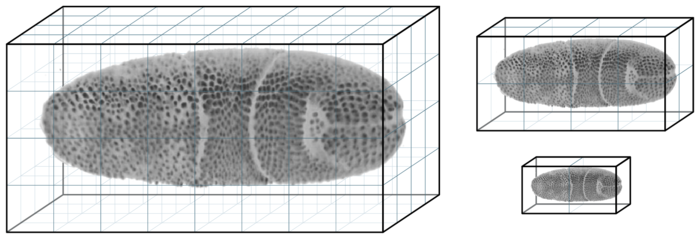
\includegraphics[width=0.6\textwidth]{figures/BdvTikz-pyramidblocks.png}
    \caption{Illustration of the BDV file format storage strategy. The image is stored over several resolution levels (multi-scale pyramid) and in chunks.}
    \label{fig:BDVchunks}
\end{figure}

There are several implementations of this strategy, for instance in Imaris\footnote{\href{http://open.bitplane.com/Default.aspx?tabid=268}{\coloredlink{IMARIS 5.5 File Format Description (IMS).}}} and with the new file format N5\footnote{\href{https://github.com/saalfeldlab/n5}{\coloredlink{N5 API on GitHub.}}} proposed by the Saalfeld lab.
Some of them are inter-compatible.
We will pick the BDV file format all along this document. 
The \Bdv has proved its value and impact on our field.
For instance our previous work on cell lineaging in large images, \wikilink{MaMuT}{MaMuT}, is based on BDV~\cite{MaMuT}.



\subsubsection{The tutorial dataset.}

Mastodon was created specially because we needed to harness very big, multi-view images. We wanted to generate  comprehensive lineages and follow a large number of cells over a very long time.
This accumulation of inflated words is tied to the very large  - in objective disk space  occupation - images we deal with using modern microscopy tools. 
Such datasets might not be optimal for a first contact with Mastodon.
So just for this tutorial we will use a smaller dataset.
It is a small region cut into a movie following the development of a drosophila, acquired in Pavel Tomancak lab (MPI-CBG).
You can find it on Zenodo\footnote{\href{https://zenodo.org/record/3336346}{\coloredlink{https://zenodo.org/record/3336346}}} there: \href{https://doi.org/10.5281/zenodo.3336346}{
\includegraphics[height=1.5\fontcharht\font`\B]{figures/zenodo3336346.png}}

It is a zip file that contains 3 files:
\begin{minted}{text}
    14M  datasethdf5.h5
   2.7K  datasethdf5.settings.xml
   8.7K  datasethdf5.xml
\end{minted}

The \texttt{.h5} file is the HDF5 file mentioned above, that contains the image data itself.
The \texttt{data\-sethdf5.xml} is a text file following the XML convention, specific to the BDV file format, that contains information about the the image data and metadata. 
When we want to open a BDV file, we point the reader to this file.
The \texttt{datasethdf5.settings.xml} is an optional file that stores user display parameters, such as channel colors, min and max display value, as well as bookmarks in the data. 
We refer you to the \wikilink{BigDataViewer\#Loading_and_Saving_Settings}{BDV documentation} about this file.
Mastodon uses this settings file to store that same information.

If you open this data in the \Bdv (in Fiji in the \menu{Plugins > BigDataViewer > Open XML/HDF5} menu), you should see something like in figure~\ref{fig:OpeningImage}. 
There is about 70 cells in each of the 30 time-points, arranged in a layer at the top of the sample. 
The deeper part of the sample (low Z coordinates) has some hazy, diffuse signal from which we cannot individualize cells.
As time progresses, the cells move towards the middle part and bottom (high Y coordinates) part of the image, and some of them move deeper in Z, initiating gastrulation.

The goal of this short tutorial is to track all these cells in Mastodon.

\begin{figure}
     \centering
         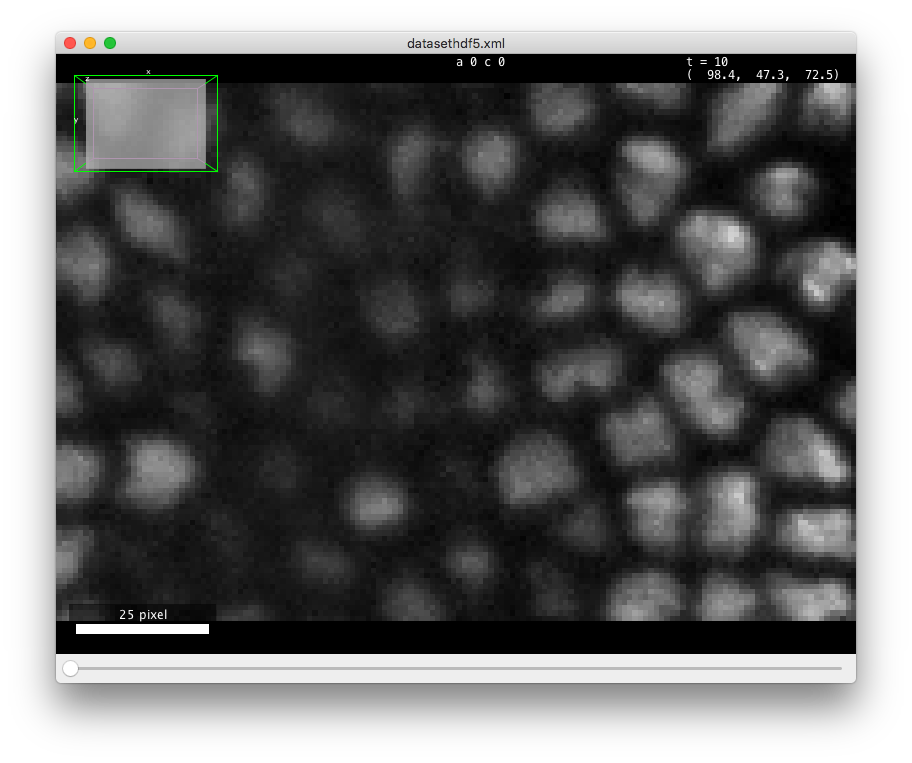
\includegraphics[width=0.3\textwidth]{figures/BDV-imageXY.png}
         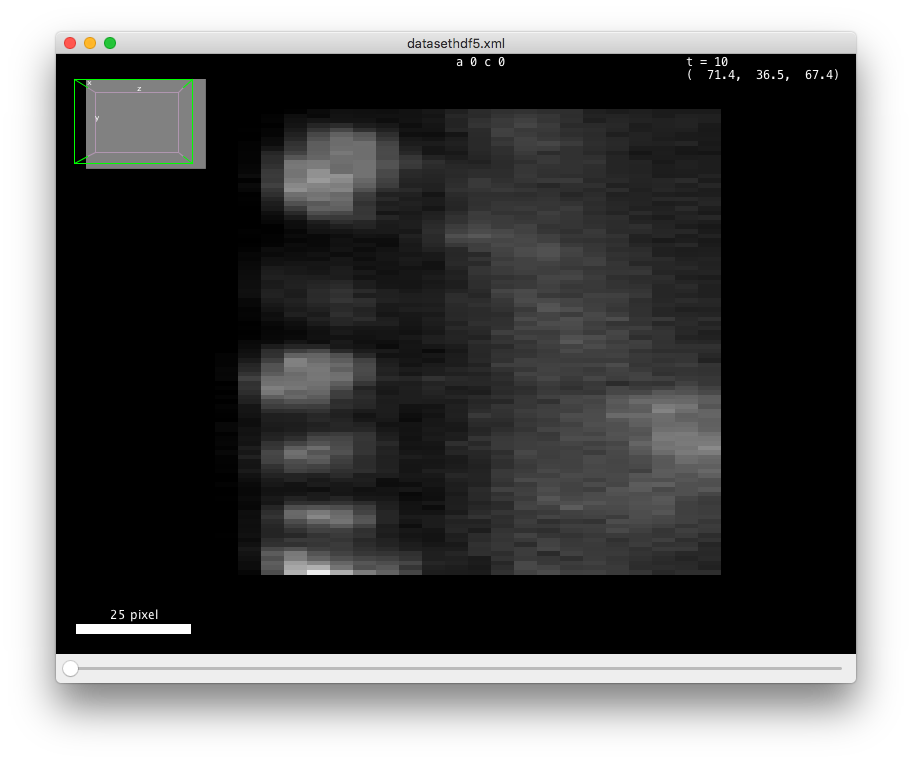
\includegraphics[width=0.3\textwidth]{figures/BDV-imageXZ.png}
         \caption{The tutorial dataset opened in \Bdv, seen along XY (left) and XZ (right)}
     \label{fig:OpeningImage}
\end{figure}  




\subsection{Getting Mastodon.}

As of today, Mastodon is available as a preview. We are still working on adding and validating features.
Nonetheless the preview has everything we need to track these cells.
Also, Mastodon is independent of ImageJ or Fiji, it can operate as a standalone software. 
However we currently distribute it via Fiji, because the updater and the dependency management are so convenient. 
So the first thing to do is to grab Fiji\footnote{\href{http://fiji.sc/}{\coloredlink{http://fiji.sc/}}}, if you do not have it already.

Then launch the \wikilink{Updater}{Fiji updater} and once your Fiji is up to date, click on the \texttt{Manage update site} button.
We will add the \wikilink{Following_an_update_site}{add the Mastodon update site}.
You should find the Mastodon preview site in the list. 
Select it, update Fiji and restart it. 
After restarting, you should find the command \menu{Plugins > Mastodon (preview)} at the bottom of the menu.

\begin{center}
    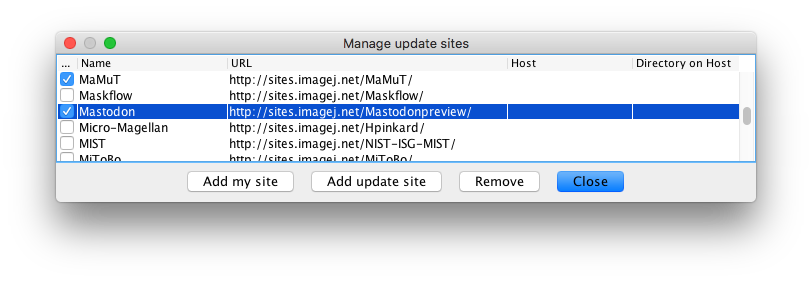
\includegraphics[width=0.7\textwidth]{figures/Mastodon_UpdateSite.png}
\end{center}



\subsection{Creating a new Mastodon project.}

After launching the command, this plain, sober window appears.
\begin{center}
         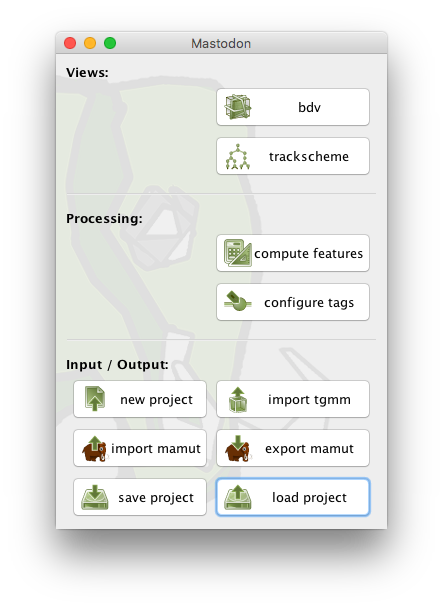
\includegraphics[width=0.3\textwidth]{figures/Mastodon_MainWindow.png}
\end{center}

Click on new \texttt{new project}, and browse to the \texttt{datasethdf5.xml} file of the XML/HDF5 file pair of the tutorial dataset.
All the buttons that were grayed out should be enabled. 
Click on the \texttt{bdv} button.
A BDV window should appear and if it does everything is right.
\begin{center}
         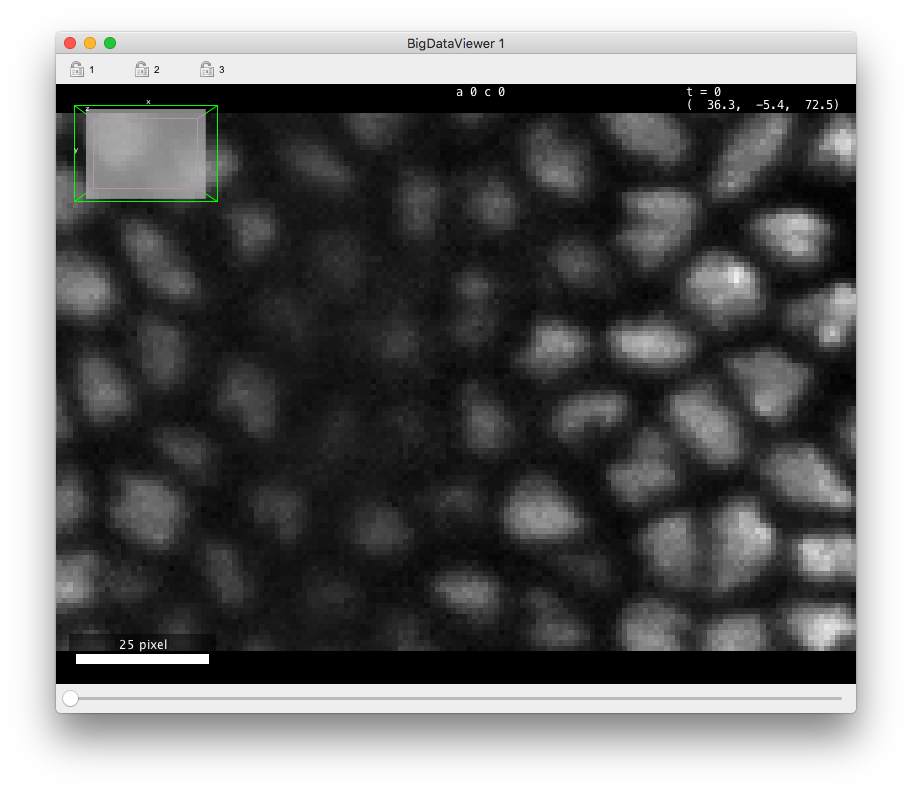
\includegraphics[width=0.4\textwidth]{figures/Mastodon_BDV.png}
\end{center}

It is almost a regular BDV window and if you already know who to use it and the key bindings you should find your marks quickly.
The BDV view displays a \textit{slice} of the image through arbitrary orientation. 
Below we give the commands and key-bindings for navigation in a Mastodon-BDV window. 
They are indeed close to what is found in the standard \Bdv but some changes. 
\textbf{Please note:} You can reconfigure almost everything in Mastodon, as we will see later, including key-bindings.
In this tutorial and the next ones, the key-bindings we present are for the \texttt{Default} configuration.
In the table~\ref{tab:MastodonBDVNavigationKeys} you will find the key bindings to navigate through the image data.

\begin{table}[!htbp]
    \centering
    
    \caption{Default navigation key-bindings for Mastodon-BDV views.}

    \begin{tabulary}{\textwidth}{L|J}
    
    \toprule
    \textbf{Action}                 & \textbf{Key}              
    \\ \midrule
    
    \multicolumn{2}{c}{\textit{View.}}
    \\ \midrule
    
    Move in X \& Y.                 & \keys{Right-click} and \keys{Drag}
    \\ \midrule
    
    Move in Z.                      & \keys{Mouse-wheel}. Press and hold \keys{\shift} to move faster, \keys{\ctrl} to move slower.
    \\ \midrule
    
    Align view with X / Y / Z axes. &  
    \begin{minipage}[t]{0.7\textwidth}
    \begin{itemize}
        \item  Align with XY plane: \keys{\shift+Z}
        \item Align with YZ plane: \keys{\shift+X}
        \item Align with XZ plane: \keys{\shift+C} or \keys{\shift+Y} 
    \end{itemize}
    The view will rotate around the location you clicked.
    \end{minipage}
    
    \\ \midrule
    
    Zoom / Unzoom.                  & \keys{\ctrl+\shift+Mouse-wheel} or \keys{\cmd+Mouse-wheel}. The view will zoom and unzoom around the mouse location.
    \\ \midrule

    \multicolumn{2}{c}{\textit{Time-points.}}
    \\ \midrule
    
    Next time-point.                & \keys{]} or \keys{M}
    \\ \midrule
    
    Previous time-point.            & \keys{[} or \keys{N}                                                                                     
    \\ \midrule

    \multicolumn{2}{c}{\textit{Bookmarks.}}
    \\ \midrule

    Store a bookmark.               & \keys{\shift+B} then press any key to store a bookmark with this key as name. A bookmark stores the position, zoom and orientation in the view but not the time-point. Bookmarks are saved in display settings file.
    \\ \midrule
    
    Recall a bookmark.              & Press \keys{B} then the key of the bookmark.
    \\ \midrule  
    
    Recall a bookmark orientation.  & Press \keys{O} then the key of the bookmark. Only the orientation of the bookmark will be restored.
    \\ \midrule
    
    \multicolumn{2}{c}{\textit{Image display.}}
    \\ \midrule
    
    Select source 1, 2 \ldots         & Press \keys{1} / \keys{2} \ldots
    \\ \midrule
    
    Brightness and color dialog.    & Press \keys{S}. In this dialog you can adjust the min \& max for each source, select to what sources these min \& max apply and pick a color for each source.
    \\ \midrule
    
    Toggle fused mode.              & Press \keys{F}. In fused mode, several sources are overlaid. Press \keys{\shift+1} / \keys{\shift+2} \ldots to add / remove the source to the view. In single-source mode, only one source is shown.
    \\ \midrule
    
    Visibility and grouping dialog.     & Press \keys{F6}. In this dialog you can define what sources are visible in fused mode, and define groups of sources for use in the grouping mode.
    \\ \midrule
    
    Save / load display settings.       & \keys{F11} / \keys{F12}. This will create a \texttt{XYZ\_settings.xml} file in which the display settings will be saved.
    \\ \bottomrule

\end{tabulary}


    \label{tab:MastodonBDVNavigationKeys}
    \vspace{-10pt}

\end{table}

Now you want to save the project. 
Go back to the main window, and click on the \menu{save project} button.
This will create a single file, called for instance \texttt{drosophila\_crop.mastodon} file. 
This file is actually a zip file that contains the tracks and \textit{links} to the image data.
The image data is kept separate from the Mastodon file, which allows for using it with another software, independently. 
So if you want to transfer or move a full Mastodon project, you need to take the \texttt{.mastodon} file and all the \texttt{.xml} and \texttt{.h5} files from the \Bdv dataset.

Next time you want to open this project, just click on the \menu{load project} button and point the file browser to the \texttt{.mastodon} file.
The image data will be loaded along with the lineages.



\subsection{Detecting cells.}

We want to track automatically all the cells in this dataset, and the first step is therefore to detect them.
Mastodon ships a wizard to perform cell detection. 
It is very much inspired by the \wikilink{TrackMate}{TrackMate} GUI, and if you know this software you will find your marks here.
Also, the algorithms are very close to what was in TrackMate~\cite{TrackMate}, but they have been heavily optimized for Mastodon.

The detection wizard can be launched from the \menu{Plugins > Tracking > Detection...} menu item. 
You should have a window like this one appearing:
\begin{center}
         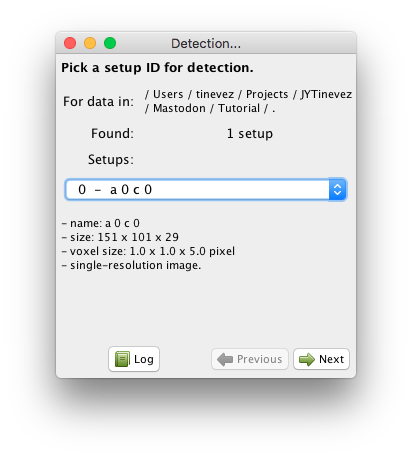
\includegraphics[width=0.4\textwidth]{figures/Mastodon_DetectionWizard_01.png}
\end{center}

Like for TrackMate, the automated tracking user interface uses \textit{wizards} to enter parameters, select algorithms, \textit{etc.}
You can navigate back and forth with the \menu{\smallimg{arrow_right.png} Next} and  \menu{\smallimg{arrow_left.png} Previous} buttons. 
The \menu{\smallimg{book.png} Log} button will bring an independent panel where all the activity in the wizard are logged as text. 

This first panel allows for selecting the target \textit{source} on which the detection will be run. 
Since we use the \bdv for images, a channel or a view is stored and displayed as a source. 
A source can have multiple resolutions stored, as explain in paragraph~\ref{BDV_advantages}, but for the data used in this tutorial this is not the case. The sources are nicknamed 'setups' in this panel.
They are numbered from 0 and can be selected from the drop-down list. 
Below the list we try to display the metadata we could retrieve from the \bdv file.
Just pick the first and only channel, and click \menu{\smallimg{arrow_right.png} Next}.

You can now choose to operate only on a rectangular ROI in the image. 
If you check the \textbf{Process only a ROI} button, new controls appear in the panel, and a ROI is drawn into an open BDV view (a new one is created if one is not opened).
The ROI is painted as a wire-frame box, green for vertices that point towards the camera from the displayed slice, and purple for vertices that points away from the camera, below the displayed slice.
The intersection of the ROI box with the displayed slice is painted with a purple semi-transparent overlay, with a white dotted line as borders.
You can control the ROI bounds wither with the controls in the panel, or by directly dragging the ROI corners in the BDV view.
Time bounds can also be set this way. In our case we want to segment the full image over all time-points, so leave the \textbf{Process only a ROI} button unchecked.

You cannot have non-rectangular ROI in Mastodon. Nonetheless they are super useful as is. 
You can for instance combine several detection steps using different parameters in different region of your image. Or different time interval.

\begin{center}
         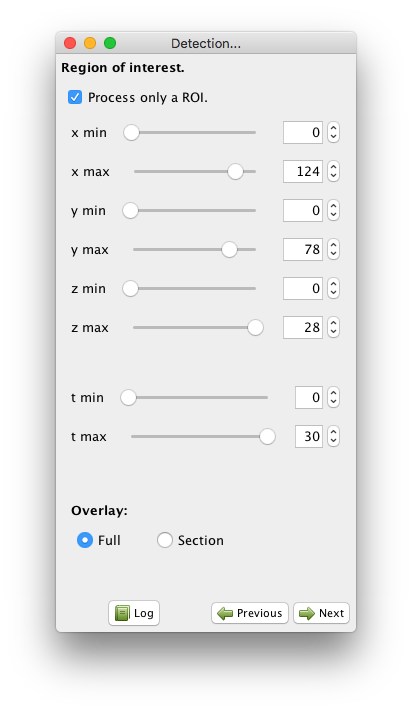
\includegraphics[height=0.25\textheight]{figures/Mastodon_ROIpanel.png}
         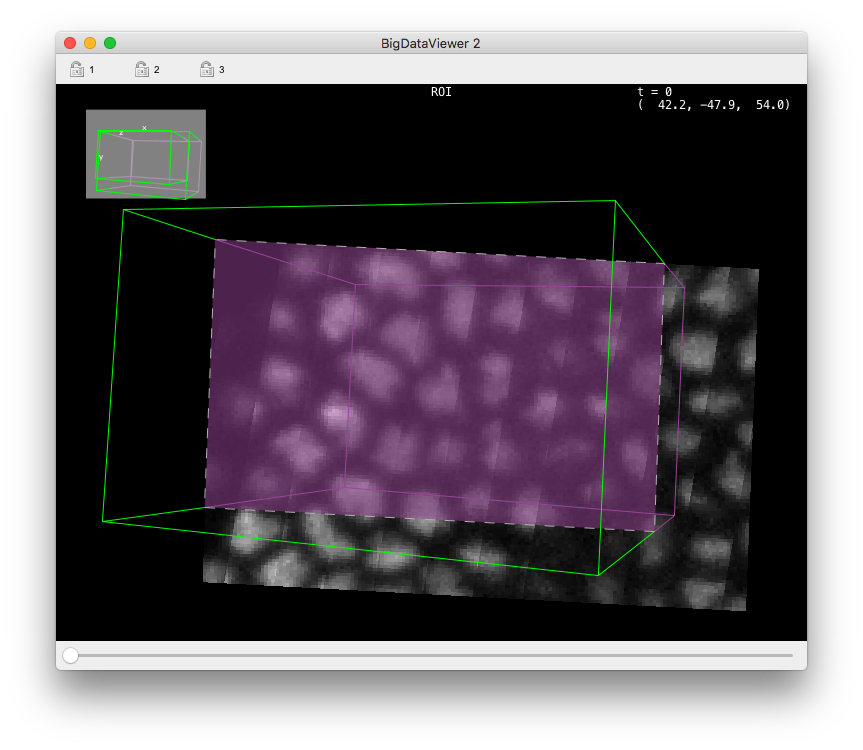
\includegraphics[height=0.25\textheight]{figures/Mastodon_ROIBDV.png}
\end{center}

The next panel lets you choose the detector you want to use.
In vanilla Mastodon, three detectors are available.
Right now, we will use the default one, the \textbf{DoG detector}, which should be good enough for most cases.
DoG means 'difference-of-Gaussians'.
It is an efficient approximation of the LoG ('Laplacian of Gaussian') filter, and there is also a detector in Mastodon based on the latter.

These detectors excel at finding roundish structures in the image that are bright over a dark background.
The structures must have a shape somewhat close to a sphere, but they can accommodate a lot of variability.
As a rule of thumb, if you can define rough estimate of the radius of these structures, they are eligible to be picked up by our detectors. 
This also implies that in Mastodon, we cannot segment complex shapes, or object labeled by their contour (\textit{e.g.} cell membranes), or even exploit these shapes to have an accurate measurements of the volume. 
This is an important limitation of Mastodon.

For now, select the \textbf{DoG detector} and click \menu{\smallimg{arrow_right.png} Next}.

Here is briefly  how it works.
The LoG detector, and its approximation the DoG detector, is the best detector for Gaussian-like particles in the presence of noise. 
It is based on applying a Laplacian of Gaussian (LoG) filter on the image and looking for local maxima. The result is obtained by summing the second order spatial derivatives of the gaussian- filtered image, and normalizing for scale.
Local maxima in the filtered image yields spot detections. 
Each detected spot is assigned a \textbf{quality} value by taking the local maxima value in the filtered image.
So by properties of the LoG filter, this quality value is larger for :
\begin{myitemize}
    \item bright spots;
    \item spots which diameter is close to the specified diameter.
\end{myitemize}

So the DoG detector requires only two parameters: the estimated diameter of the object we want to detect, and a threshold on the quality value, that will help separating spurious detections from real ones. 
The panel you are presented let you specify these parameters, and preview the resulting detection.
Try with 10 pixels for \textbf{Estimated diameter} and 0 for the \textbf{Quality threshold}.
The click on the \menu{\smallimg{led-icon-eye-green.png} Preview} button.
A preview panel should open shortly, showing detection results on the current frame

\begin{center}
         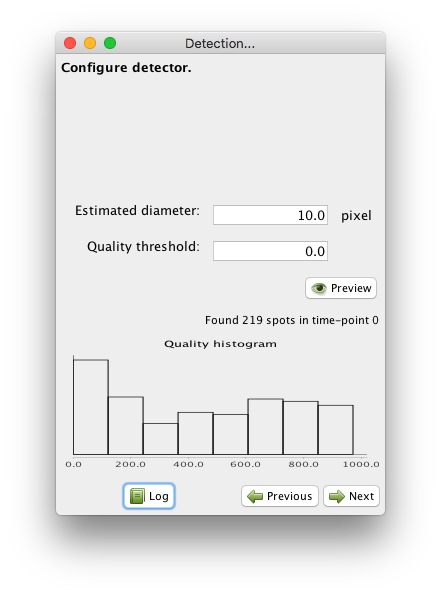
\includegraphics[height=0.25\textheight]{figures/Mastodon_DoGconfig1.png}
         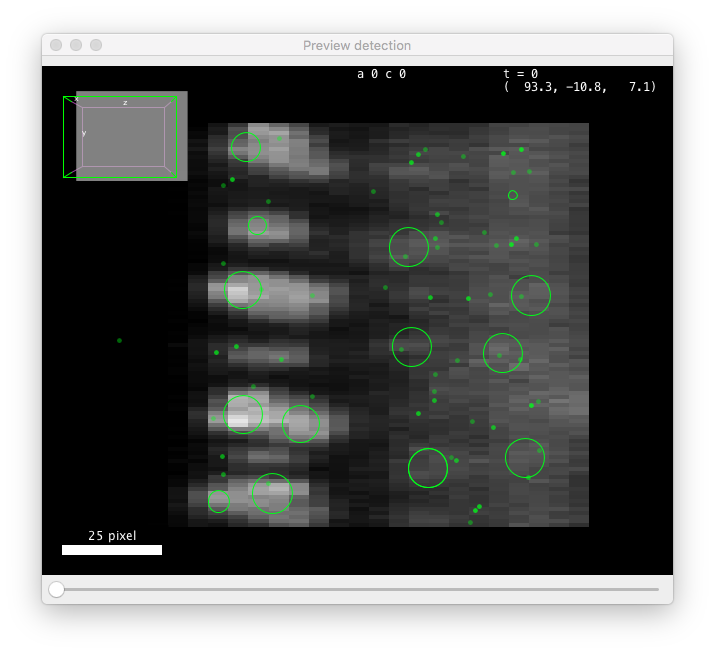
\includegraphics[height=0.25\textheight]{figures/Mastodon_DoGconfig2.png}
\end{center}

These values are close but not quite.
You can see that the diameter value is too small to properly grasps the elongated shape of the cells along Z (the BDV view on the left panel above is rotated to show a YZ plane). 
Also the threshold value is too low, and some spurious detections are found below the epithelium.
These spots have a low quality, that manifests as a peak at low value in the quality histogram displayed on the configuration panel.
From the shape of the histogram, we can infer that a threshold value around 100 should work.
However we also need to change the diameter parameter, which will change the range of quality values.
After trial and errors, values around 15 pixels for the diameter and 400 for the threshold seem to work.

Note that you can run the preview on any frame.
You just have to move the time slider on the preview window.
Once you are happy with the parameters, click on the \menu{\smallimg{arrow_right.png} Next} button.
All the frames specified in the ROI (if any) will be processed. 
In our case it should conclude quickly and the following panel should appear:

\begin{center}
         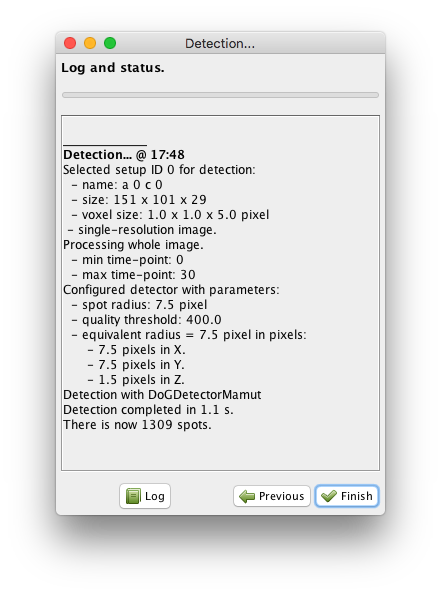
\includegraphics[height=0.25\textheight]{figures/Mastodon_DetectionResuts.png}
\end{center}

We now have more than 1000 cells detected and this concludes the detection step.
Click on the \menu{\smallimg{accept-icon.png} Finish} button, and the wizard will disappear.

If you have complex images mixing several size of objects, or detection parameters that work for one part of the movie but not for another one, you could restart a new detection now, selecting for instance other parts of the movie with the ROI.
You can do this and more, but for this kind of approach, the \textbf{Advanced DoG detector} offers more configuration capabilities, that will review later.



\subsection{Linking cells.}

What we just did is the detection step. 
It yields one Mastodon spot per cell, but the notion of cell identity propagated over time is missing yet.
The particle linking step just does that.
A particle linking or tracking algorithm accepts a collection of spots, ordered by frames (time-points), and tries to link each spot to the next spot(s) in the next frame or so. 
All the spots you can reach by starting from one spot and navigating across links build a \textit{track}, and in our case it represents one cell (or any other object) followed over time. 
In most cases there is one spot per frame for a track, meaning that that a spot has at most one incoming link (spot from previous frame) and one outgoing kink (spot in next frame). 
But some algorithms can accommodate \textit{e.g.} dividing cells (2 outgoing links for the mother cell going to the two daughter cells) and merging events. There is a vast literature behind tracking algorithms, and it is an active domain of Research. A relatively recent paper compare implementation and list some pros and pitfalls of many of them~\cite{Chenouard2014}.

\begin{wrapfigure}{r}{0.3\textwidth}
    \centering
    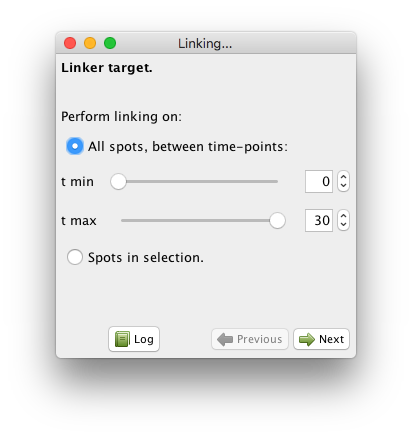
\includegraphics[height=0.3\textwidth,trim=0.5cm .5cm .5cm .5cm,clip]{figures/Mastodon_LinkingWizard_01.png}
\end{wrapfigure}

Like for the detection step, linking in Mastodon happens in a wizard.
And also like for detection, the linking algorithms currently available in Mastodon are adapted from TrackMate. 

Launch the wizard from the GUI, with the \menu{Plugins > Tracking > Linking...} menu item. 
The first panel you are shown lets you select what spots to include in linking. 
There are two modes:
\begin{myitemize}
    \item Either you take all the spots between a start and and end frame. By default, all frames are selected.
    \item Either you specify you want to link only the spots that are in the selection. 
    This mode offers a lot of flexibility when facing complicated cases. 
    It is best use along with the selection creator, that we will introduce later in this manual.
\end{myitemize}
For now, just leave the parameters as they are, which will include all spots in the linking process, and click next.
You can now choose between several linking algorithms. 
In Mastodon, they fall mainly in two categories.

The first two LAP trackers are based on the \textbf{Linear Assignment Problem (LAP) framework}, first developed by Jaqaman \textit{et al.}~\cite{Jaqaman2008}, with important differences from the original paper described elsewhere~\cite{TrackMate}. We focused on this method for it gave us a lot of flexibility and it can be configured easily to handle many cases. You can tune it to allow splitting events, where a track splits in two, for instance following a cell that encounters mitosis. Merging events are handled too in the same way. More importantly are gap-closing events, where a spot disappear for one frame (because it moves out of focus, because detection failed, ...) but the track manages to recuperates and connect with reappearing spots later.

In Mastodon the LAP algorithms exists in two flavors: a simple one and a not simple one. There are again the same, but the simple ones propose fewer configuration options and a thus more concise configuration panel. In short:
\begin{myitemize}
    \item The simple one only allows to deal with gap-closing events, and prevent splitting and merging events to be detected. Also, the costs to link two spots are computed solely based on their respective distance.
    
    \item The not simple one allows to detect any kind of event, so if you need to build tracks that are splitting or merging, you must go for this one. If you want to forbid the detection of gap-closing events, you want to use it as well. Also, you can alter the cost calculation to disfavor the linking of spots that have very different feature values.
\end{myitemize}



\newpage
\section{Manually editing tracks in Mastodon. TrackScheme.}

One of the key feature of Mastodon, the implementation of which made our lives extremely hard and rich, is the ability to edit manually at any time any spot or link within an annotation that can contains billions of them, while retaining a good and pleasant response time from the software.
I am not even speaking of the undo/redo mechanism, which getting right was also very interesting. 

In this tutorial, we will show how to do just that, from existing tracking data, the one we generated in the previous section. 
We will use it as an opportunity to present \TrackScheme, the track visualizer of Mastodon, as well as introduce several useful editing features such as the undo/redo mechanism mentioned above.
We will also introduce the various visual hints that help the user knowing what spot or link is currently edited or inspected, such as the \textbf{focus}, the \textbf{highlight} and the \textbf{selection}.

Manual editing is often \textbf{not desirable}, first because it is not objective which might be detrimental in situations where the performance of an algorithm is evaluated, or when an unknown motion characteristics is investigated. 
Second, because it does not look like a realistic solution when \textit{e.g.} thousands of cells are to be followed over thousands of time-points.
Regarding the latter however, several courageous individuals sacrificed their time, energy and sometimes sanity in doing so, for the sake of finally getting a scientific answer when there was no other working solutions. 
See for instance~\cite{MaMuT} and~\cite{McDole2018}.
If you are going this way, Mastodon aims at providing tools to do so, in the hopefully fastest and least painful way possible. 
Also, you can combine the fully automated approach of the previous chapter with manual editing to correct hopefully a few numbers of mistakes.
Finally, there is also a semi-automated tracking tool, that we will introduce later.

This tutorial will start by presenting you the manual editing tools of Mastodon, as well as \TrackScheme and the focus, highlight and selection tools.
Because this catalogue of actions can be a bit dry and long to swallow, we will in the last paragraph use it to remove and rebuild some tracks from the results of the last tutorial.



\subsection{TrackScheme, the lineage view and editor.}

First, load or retrieve the tracking data of the previous chapter. 
You should have a few hundreds of tracks. 
To open a TrackScheme view window, press the \menu{trackscheme} button on the main window (Figure~\ref{fig:MastodonMainWindow} page~\pageref{fig:MastodonMainWindow}).
A window as shown in Figure~\ref{fig:TrackScheme} should open.

\begin{figure}
    \centering
    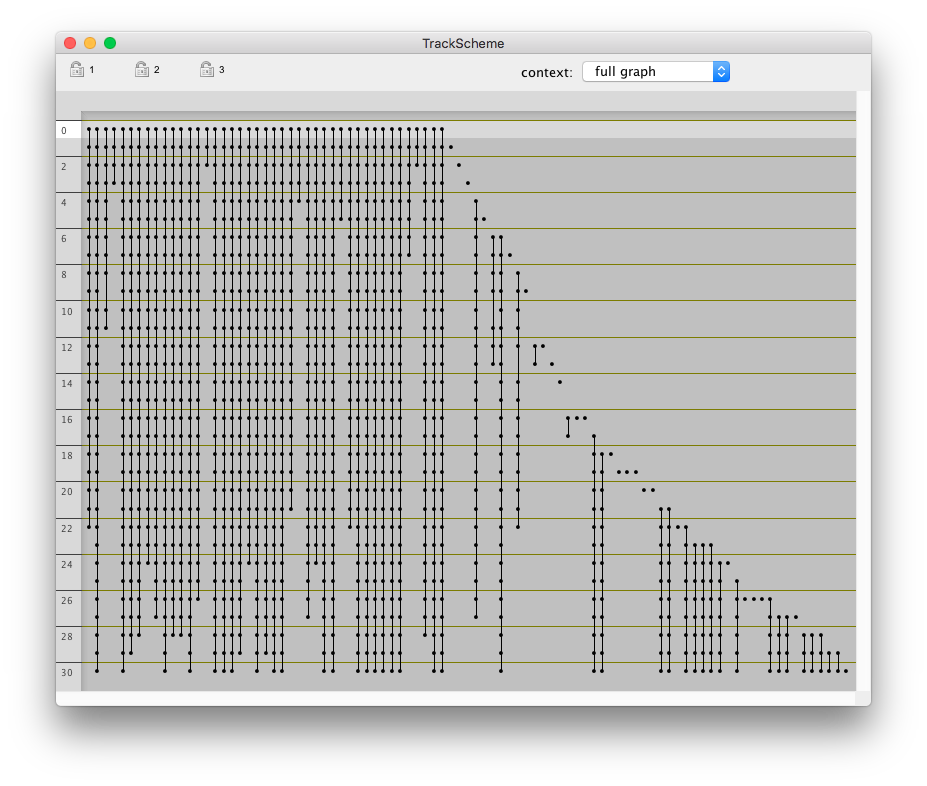
\includegraphics[width=0.8\textwidth,trim=0.5cm .5cm .5cm .5cm,clip]{figures/Mastodon_TrackScheme.png}
     \caption{The TrackScheme window.}
     \label{fig:TrackScheme}
\end{figure}  

The TrackScheme view offers a special way of displaying tracks. 
If you are familiar with TrackMate, you will see that we brought the same kind of features here, but scaled to large data.
You can think of TrackScheme as a workbench for tracks, where you will edit, cut, stitch and rename them.
It displays a kind of "track map", where a track is laid on a panel, arranged vertically over time, as a Parisian subway train map. 
Tracks are displayed hierarchically, discarding the spatial location of each spot. 
Each track is laid out going through time from top to bottom.
One horizontal line corresponds to a single time-point in the movie.
One vertical column corresponds to a single track, that is all the spots that are connected by links over time, including divisions and merges.
It is a great tool particularly to study and edit cell lineages.

When opened, the view in TrackScheme is scaled so that the full data is shown, all tracks over all time-points. 
Even on our small dataset, most of the tracks and spots appear as single lines or dense boxes.
To see the details of each track, you need to zoom in and navigate around the data.
The navigation actions their mappings are listed in the Table~\ref{tab:MastodonTrackSchemeNavigationKeys} below.

\begin{table}[!htbp]
    \centering
    \caption{Default navigation key-bindings for Mastodon-TrackScheme views.}
    \begin{tabulary}{\textwidth}{L|J}
    
    \toprule
    \textbf{Action}                 & \textbf{Key}              
    \\ \midrule
    
    \multicolumn{2}{c}{\textit{View.}}
    \\ \midrule
    
    Move around.                    & \keys{Right-click} and \keys{Drag} or \keys{Mouse-wheel}
    \\ \midrule
    
    Zoom / unzoom in X.             & \keys{\shift+Mouse-wheel}
    \\ \midrule
    
    Zoom / unzoom in Y.             & \keys{\ctrl+Mouse-wheel}
    \\ \midrule
    
    Zoom / unzoom in X \& Y.         & \keys{\ctrl+\shift+Mouse-wheel}
    \\ \midrule

    Full zoom, full unzoom.         & Press \keys{Z}. The view zoom at max level to the mouse location. Pressing  \keys{Z} again to unzoom fully.
    \\ \midrule
    
    Zoom in a box.                  & Press and hold \keys{Z} then drag a box. The view will zoom to the box.                            
    \\ \bottomrule

\end{tabulary}

    \label{tab:MastodonTrackSchemeNavigationKeys}
\end{table}

Try to zoom in until you can see the label of a few spots.
TrackScheme implements adaptive level of details depending on the zoom level, so that we can accommodate plotting a large amount of data without compromising the responsiveness of Mastodon too much (Figure~\ref{fig:TrackSchemeZoomLevel}).
On the finer level of details, spots are plotted as circles, with the spot label shown.
As you zoom out, they becomes just empty circles, then points, then they disappear to only show the track as a line.
When the zoom level is so low that several tracks coalesce, they are drawn as a gray box. 

\begin{figure}
    \centering
    \subfloat[]{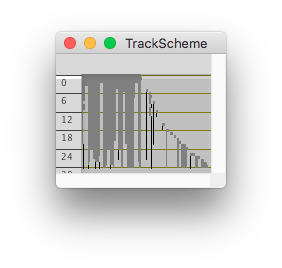
\includegraphics[width=0.25\textwidth,trim=0.5cm .5cm .5cm .5cm,clip]{figures/Mastodon_TrackScheme_Zoom_0.png}}
    \subfloat[]{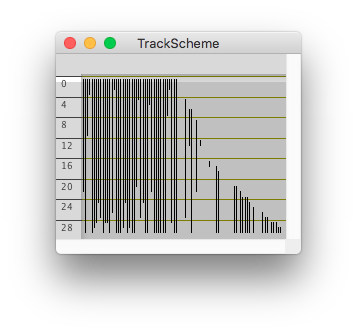
\includegraphics[width=0.35\textwidth,trim=0.5cm .5cm .5cm .5cm,clip]{figures/Mastodon_TrackScheme_Zoom_1.png}}
    \subfloat[]{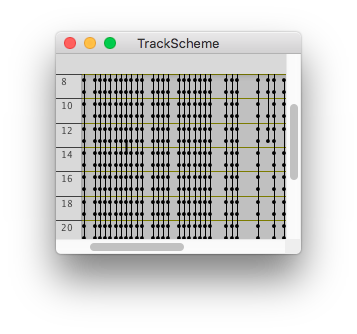
\includegraphics[width=0.35\textwidth,trim=0.5cm .5cm .5cm .5cm,clip]{figures/Mastodon_TrackScheme_Zoom_2.png}}
    \\
    \subfloat[]{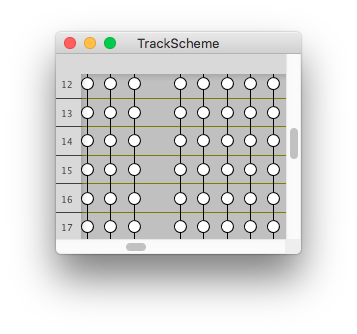
\includegraphics[width=0.35\textwidth,trim=0.5cm .5cm .5cm .5cm,clip]{figures/Mastodon_TrackScheme_Zoom_3.png}}
    \subfloat[]{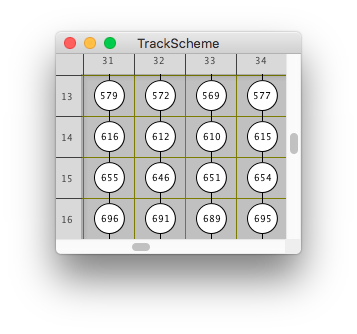
\includegraphics[width=0.35\textwidth,trim=0.5cm .5cm .5cm .5cm,clip]{figures/Mastodon_TrackScheme_Zoom_4.png}}
    
    \caption{TrackScheme displays spots and links differently depending on the zoom level. \textbf{a.}~At low zoom level tracks that coalesce are shown as gray boxes. \textbf{b.}~Zooming in, the individual tracks appear first as black lines. \textbf{c.}~When they are separated enough, spots appear as black dots. \textbf{d.}~With an even higher zoom level they are shown as empty circles. \textbf{e.}~Until they grow big enough so that the spot labels can be painted. Notice the size of the sliders at the bottom and at the right of the view.}
    \label{fig:TrackSchemeZoomLevel}
\end{figure}  

\subsection{The focus and the spot labels.}

You probably noticed that some spots are painted differently from their neighbors. 
Mastodon manages three special collections of spots and links to facilitate making sense of the data across views:
\begin{myitemize}
    \item the \textbf{selection}, painted in green, that manages a classical selection of spots and links;
    \item the \textbf{highlight}, used to highlight the spot or link currently under the mouse;
    \item the \textbf{focus}, particularly used in TrackScheme, to indicate what spot is currently focused on by the keyboard interaction.
\end{myitemize}

\noindent We will first present the focus (see Table~\ref{tab:MastodonTrackSchemeFocusKeys}). 

\begin{table}[htbp]
    \centering
    \caption{Default key-bindings for the focus in TrackScheme and BDV views.}
    \begin{tabulary}{\textwidth}{L|J}
    
    \toprule
    \textbf{Action}                 & \textbf{Key}              
    \\ \midrule
    
    \multicolumn{2}{c}{\textit{Navigation with the Focus.}}
    \\ \midrule
    
    Follow a spot across time within a track with the focus.      & \keys{\arrowkeyup} and \keys{\arrowkeydown}
    \\ \midrule

    Jump to the beginning of a branch.                              & \keys{\Alt + \arrowkeyup}
    \\ \midrule
    
    Jump to the end of a branch.                                    & \keys{\Alt + \arrowkeydown}
    \\ \midrule

    Jump to the beginning of another branch.                              & \keys{\ctrl + \Alt + \arrowkeyup}
    \\ \midrule

    Jump to the end of another branch.                                    & \keys{\ctrl + \Alt + \arrowkeydown}
    \\ \midrule
    
    \multicolumn{2}{c}{\textit{Focus in TrackScheme.}}
    \\ \midrule
    
    Move the focus around from one track or one track branch to another.  & \keys{\arrowkeyleft} and \keys{\arrowkeyright}
    \\ \midrule
    
    Edit the label of the focused spot.             & \keys{\return}
    \\ \bottomrule
  
\end{tabulary}

    \label{tab:MastodonTrackSchemeFocusKeys}
\end{table}


\subsubsection{Moving the focus.}

The spot that has the focus is painted with a dashed contour (Figure~\ref{fig:FocusedSpots}, left). 
Only one spot can have the focus and it is set by mouse or keyboard interaction.
Click on one spot in TrackScheme when fully zoomed, and move across track and time with the arrow cursor keys \keys{\arrowkeyleft} \keys{\arrowkeyright} \keys{\arrowkeyup} and \keys{\arrowkeydown}.
If the focus reaches the border of the window, the view will be moved to follow it.
You can think of the focus as the caret in a text editor. 
It is meant to facilitate keyboard interaction.

You can also jumps across branches.
A branch in a track is a linear section of the track between divisions, fusions or the track end or start.
\keys{\Alt+\arrowkeyup} and \keys{\Alt+\arrowkeydown} will move the focus to the branch start and end.
In the case where you could navigate to several branches, for instance you are currently at a cell division and you can go the end of either daughter cells branches, you can navigate to one or the other with \keys{\Alt+\arrowkeydown} or \keys{\ctrl+\Alt+\arrowkeydown}.


\begin{figure}
    \centering
    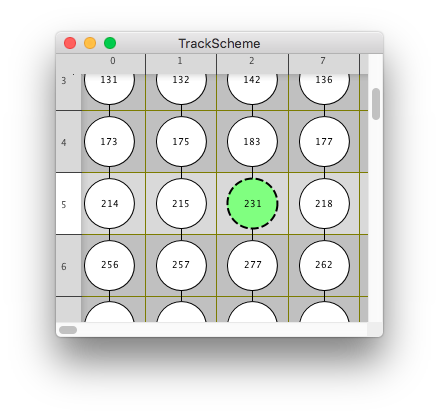
\includegraphics[height=0.25\textheight,trim=0.5cm .5cm .5cm .5cm,clip]{figures/Mastodon_FocusInTrackScheme.png}
    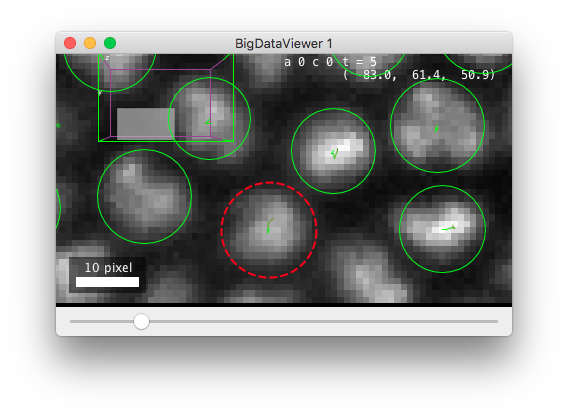
\includegraphics[height=0.25\textheight,trim=0.5cm .5cm .5cm .5cm,clip]{figures/Mastodon_FocusInBDV.png}
    \caption{Focused spots are painted in TrackScheme (left) and in BDV (right) views as ellipses with a dashed-contour.}
     \label{fig:FocusedSpots}
\end{figure}  

\subsubsection{Editing the spot labels.}

By the way, the focus is used to rename individual spots.
Zoom in so that we can see the label of the spots and move the focus to a spot. 
Press \keys{\return}.
A small editing box appears inside the spot and lets you change its label (Figure~\ref{fig:EditSpotLabel}).

By default the spot label display the spot ID. 
If you edit the label then it shows the new label you entered.
Editing the label of a spot does not affect its ID or any other properties. 
The spot label is just a convenient text field that you can use to annotate cells and search them later.
Only the spots have a label. 
The links don't.

\begin{figure}
    \begin{minipage}{.35\textwidth}
        \centering
        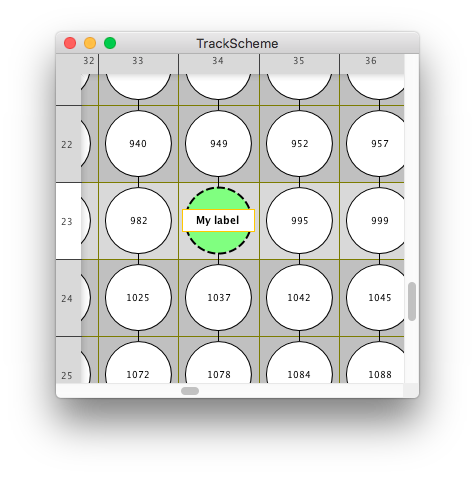
\includegraphics[height=0.22\textheight,trim=0.5cm .5cm .5cm .5cm,clip]{figures/Mastodon_EditSpotLabel.png}
        \caption{Editing a spot label in \TrackScheme.}
        \label{fig:EditSpotLabel}
    \end{minipage}
    \hfill
    \begin{minipage}{.55\textwidth}
        \centering
        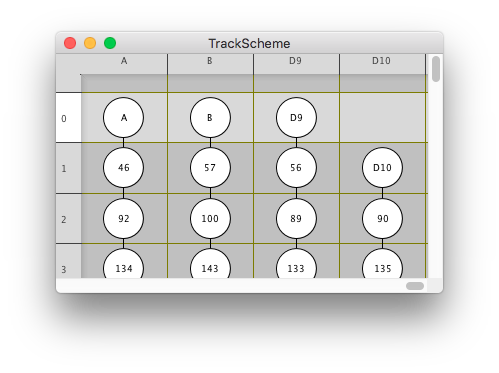
\includegraphics[height=0.25\textheight,trim=0.5cm .5cm .5cm .5cm,clip]{figures/Mastodon_TrackSchemeTrackOrder.png}
        \caption{The left to right order of tracks in TrackScheme. Track names are set by the label of their first spot in time, regardless of the time-point this spot is in. Tracks are then laid out by alphanumerical order of the track label.}
        \label{fig:TrackOrder}
    \end{minipage}
\end{figure}  


\subsubsection{The order of tracks in TrackScheme.}

The spot labels also control how the tracks are ordered in TrackScheme.
We said before that in TrackScheme all the spatial information is discarded. 
However the tracks are laid out in a deterministic order.
This order is set by the label of of a track. 

There is no special structure to follow individual tracks in Mastodon. 
For this, we simply use the first spot of a track. 
So when we speak of the label of a track, we simply means the label of the first spot (in time) in the track. 
The tracks are arranged from left to right following the alphanumerical order of the track labels.
So you can change the tracks arrangement by editing theirs first spot's label.
For instance a track named \texttt{A} will be laid out to the left of a track named \texttt{B}, and a track named \texttt{D9} will be put to the left of a track named \texttt{D10} (Figure~\ref{fig:TrackOrder}).

If you change the track labels now, the tracks will not move immediately in TrackScheme.
For the new arrangement to happen, you need to either open another TrackScheme window, or to edit the data, which we will see soon.


\subsubsection{The focus in BDV views.}

The focus also works in the BDV views.
In these views, the spot that has the focus is also painted with a thick dashed circle (Figure~\ref{fig:FocusedSpots}, right).
Parenthetically, notice that the focus is shared across all opened views. 
If you have a TrackScheme view and a BDV view opened, and that they both contain a display of the same spot, setting the focus in one view will update this very spot display in the other views.

When you are in a BDV view and have set the focus, you can also navigate with the arrow keys.
After clicking inside a cell, you can navigate in time and follow a cell lineage through the movie with \keys{\arrowkeyup} and \keys{\arrowkeydown}.
If you reach the border of the view or if the cell moves in Z, the view will be translated to keep the cell in focus.
However, you cannot edit the spot labels in a BDV view nor jump from one track to another with \keys{\arrowkeyleft} \keys{\arrowkeyright}.
Navigating across branch with \keys{\Alt+\arrowkeyup} and \keys{\Alt+\arrowkeydown} \etc also works.


\subsection{Synchronizing several views together.}
\label{sec:LinkingViews}

You probably noticed that both BDV and \TrackScheme views have a toolbar on the of the view itself.
This toolbar can be hidden and shown by a press of the \keys{T} key.
In both view types, the toolbar contains 3 gray locks \smallimg{lock_open_grey.png}, that are used to link several views together for navigation.
For instance, if you click on the lock 1 \smallimg{lock.png} on a BDV view and the same lock on a \TrackScheme view, they will be synchronized.
If you move with the focus in the \TrackScheme view, the BDV view will be translated to show the focused spot.
If you \keys{Double-click} on a spot in any view, all views in sync will translate to show the spot.
This is very handy to navigate around in TrackScheme, for instance following a cell over time while the BDV view displays where it is in the sample. 
You can even combine several BDV views in sync at different magnification to have both an overview of the cell position in the sample and a close view of the cell itself (Figure~\ref{fig:ViewsInSync}).


\begin{figure}
    \centering
    \subfloat{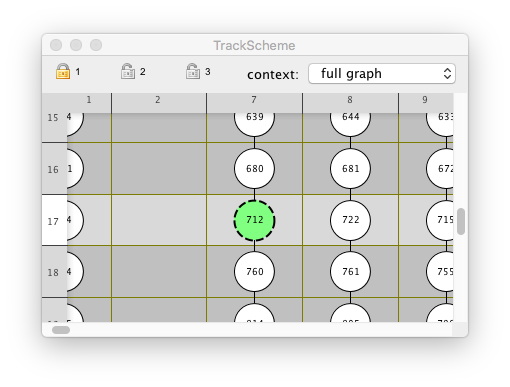
\includegraphics[height=0.18\textheight,trim=0.5cm .5cm .5cm .5cm,clip]{figures/Mastodon_Sync1.png}}
    \hfill
    \subfloat{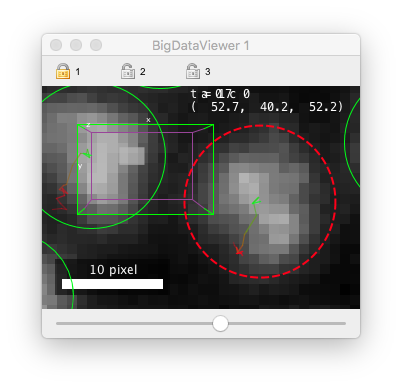
\includegraphics[height=0.18\textheight,trim=0.5cm .5cm .5cm .5cm,clip]{figures/Mastodon_Sync2.png}}
    \hfill
    \subfloat{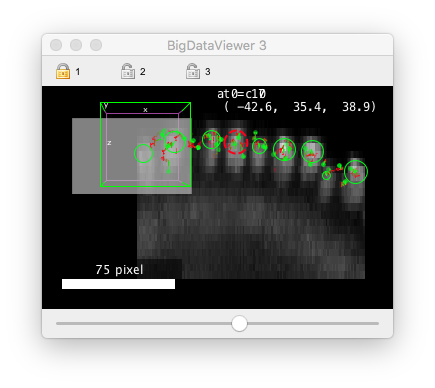
\includegraphics[height=0.18\textheight,trim=0.5cm .5cm .5cm .5cm,clip]{figures/Mastodon_Sync3.png}}
    
    \caption{Three views of the same dataset in sync. Notice that the lock number 1 is activated on the three views (in yellow). The second view is zoomed in a XY plane. The third view is dezoomed and align with XZ.}
    \label{fig:ViewsInSync}
\end{figure}  


\subsection{The highlight.}

The highlight is the second visual hint we will introduce. 
You probably already noticed it and used it: the display of spots and links that are just below the mouse cursor changes.
Highlighted spots and links are painted with a thick continuous line (Figure~\ref{fig:Highlight}). 
To highlight a spot or link you just have to lay the mouse over it.
As for the focus, the highlight is common to all views, and if you highlight a spot or a link in a view, its display is changed in all the views that show it.


\subsection{Deleting individual spots and links.}

The highlight is especially important for track editing. 
The commands that delete a single object are actually applied to the highlighted spot or link.
For instance, to delete a spot or a link in \TrackScheme, simply move the mouse cursor over it so that it is highlighted and press \keys{D}.
You should see the tracks being rearranged following the deletion. 
In a BDV view, the highlight and deletion mechanism is the same. 


\begin{figure}
    \centering
    \subfloat{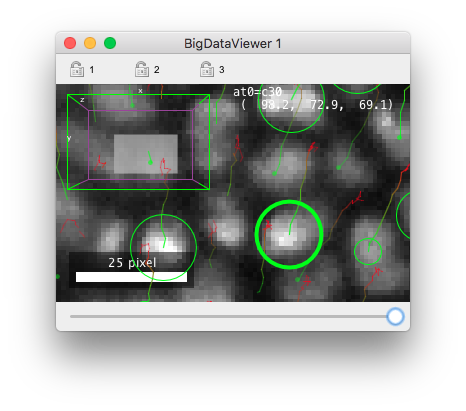
\includegraphics[height=0.14\textheight,trim=0.5cm .5cm .5cm .5cm,clip]{figures/Mastodon_HighlightSpotBDV.png}}
    \hfill
    \subfloat{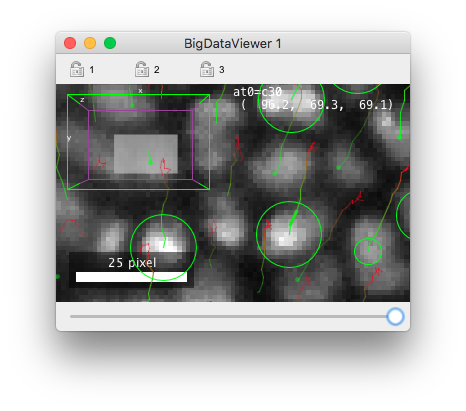
\includegraphics[height=0.14\textheight,trim=0.5cm .5cm .5cm .5cm,clip]{figures/Mastodon_HighlightLinkBDV.png}}
    \hfill
    \subfloat{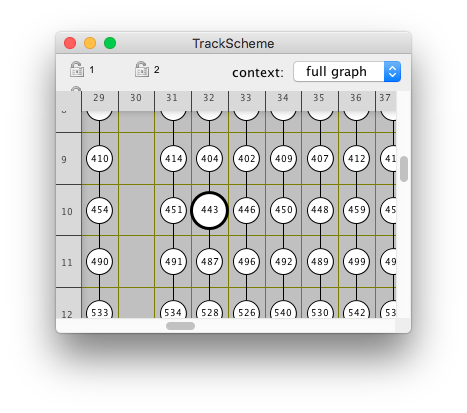
\includegraphics[height=0.14\textheight,trim=0.5cm .5cm .5cm .5cm,clip]{figures/Mastodon_HighlightSpot.png}}
    \hfill
    \subfloat{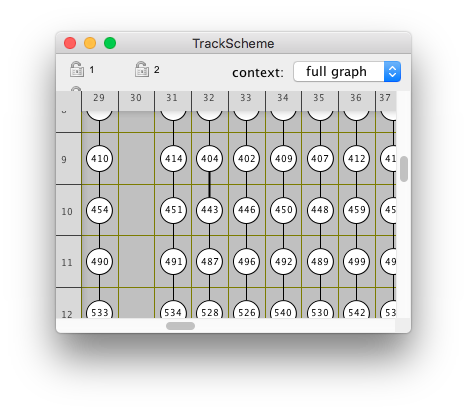
\includegraphics[height=0.14\textheight,trim=0.5cm .5cm .5cm .5cm,clip]{figures/Mastodon_HighlightLink.png}}
    
    \caption{The highlight in Mastodon. The highlighted spot or link will appear painted with a thicker line, both in the BDV and TrackScheme views.}
    \label{fig:Highlight}
\end{figure}  





\subsection{Linking spots together.}

Creating links between existing spots happens in a similar way, except that you have to point to a source spot and another target spot for a single link.
In \TrackScheme, move inside a spot until it is highlighted (no mouse-click).
You must be at a zoom level large enough so that a spot is at least painted as a dot or a circle (Figure~\ref{fig:TrackSchemeZoomLevel}c, d, e). 
Then press and hold the \keys{L} key.
Without releasing the \keys{L} key, move the mouse out of the spot.
You should see a red line representing the link to create (Figure~\ref{fig:TrackSchemeManualLink}).
Move the mouse to the desired target spot, until it becomes highlighted.
The red line should snap to it and become thicker.
If you now release the \keys{L} key now, a new link between the source and target spot is created and in TrackScheme it should cause a rearrangement of the tracks.
Notice that you cannot add a link between spots in the same frame.
Also notice that you can toggle links this way.
If you draw a link between two spots that are already connected, their link will be removed.

In BDV views, it is again very similar (Figure~\ref{fig:BDVManualLink}).
Move the mouse over a spot until it is highlighted then press and hold the \keys{L} key.
The view will automatically move to the next frame. 
The link to create will be painted as a white line, and the ghost shape of the source spot is painted as a dashed white ellipse. 
Move the mouse to the target spot in this frame until it is highlighted, then release the \keys{L} key.
The link is created.
If you press \keys{\shift+L} in a spot, the BDV view will move to the \textbf{previous} frame, and create a backward link.

You cannot move in Z while creating a link this way. 
You must orient the BDV view so that the source and target spot are roughly in the same displayed slice. 
However you can move in time. 
While still holding the \keys{L} key, press the \keys{N} or \keys{[} and \keys{M} or \keys{]} key to navigate backward and forward in time.
This way you can create links between spots separated by more than one time-point.



\begin{figure}
    \centering
    \null\hfill
    \subfloat{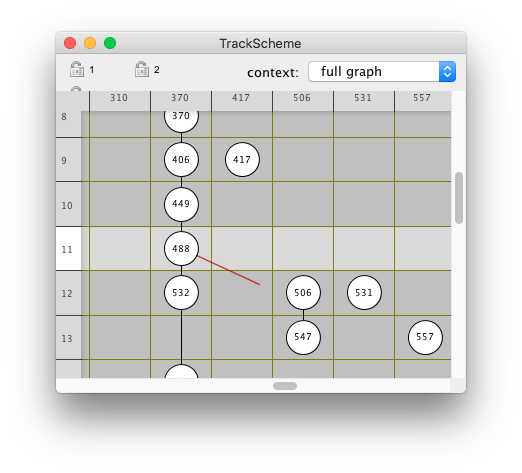
\includegraphics[width=0.3\textwidth,trim=0.5cm .5cm .5cm .5cm,clip]{figures/Mastodon_TrackSchemeManualLinking1.png}}
    \hfill
    \subfloat{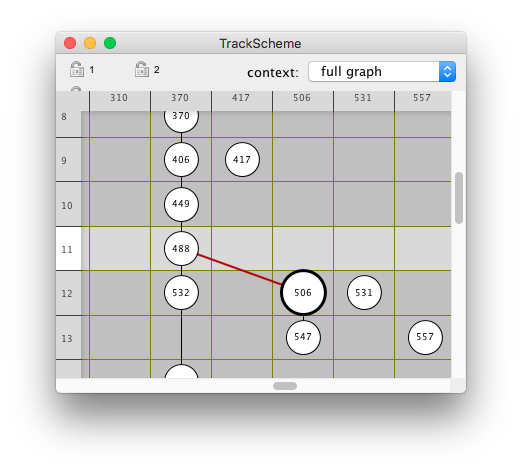
\includegraphics[width=0.3\textwidth,trim=0.5cm .5cm .5cm .5cm,clip]{figures/Mastodon_TrackSchemeManualLinking2.png}}
    \hfill
    \subfloat{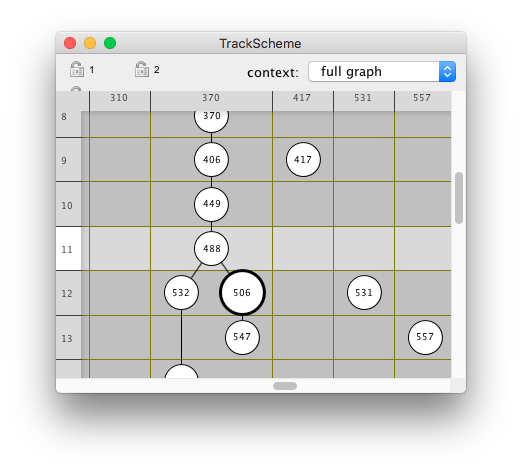
\includegraphics[width=0.3\textwidth,trim=0.5cm .5cm .5cm .5cm,clip]{figures/Mastodon_TrackSchemeManualLinking3.png}}
    \hfill\null
    
    \caption{Manually creating links in TrackScheme. Press and hold \keys{L} while hovering the mouse over a spot. Then drag the link in red to the target spot. A new link will be created between the two spots when you release \keys{L}. Doing this between two spots that are already connected removes the link between them.}
    \label{fig:TrackSchemeManualLink}
\end{figure}  


\begin{figure}
    \centering
    \null\hfill
    \subfloat{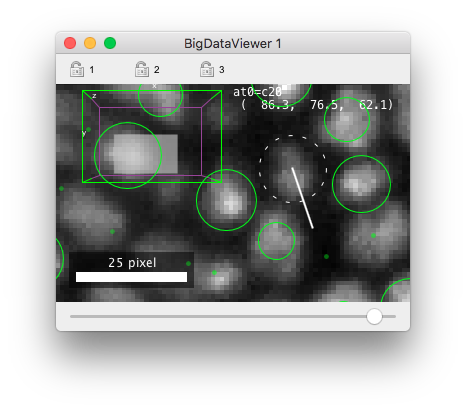
\includegraphics[width=0.3\textwidth,trim=0.5cm .5cm .5cm .5cm,clip]{figures/Mastodon_BDVManualLinking1.png}}
    \hfill
    \subfloat{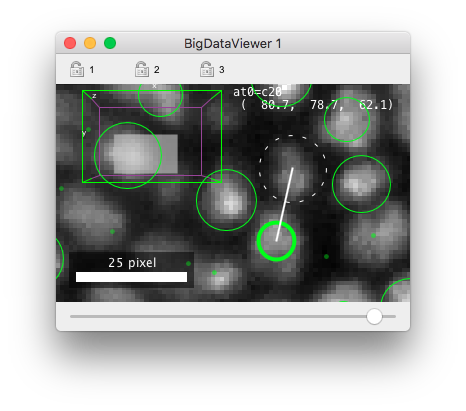
\includegraphics[width=0.3\textwidth,trim=0.5cm .5cm .5cm .5cm,clip]{figures/Mastodon_BDVManualLinking2.png}}
    \hfill
    \subfloat{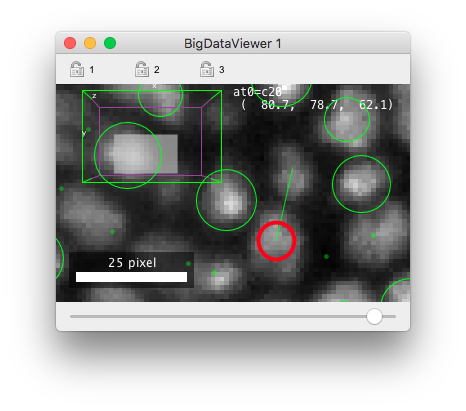
\includegraphics[width=0.3\textwidth,trim=0.5cm .5cm .5cm .5cm,clip]{figures/Mastodon_BDVManualLinking3.png}}
    \hfill\null
    
    \caption{Manually creating links in BDV views. Press and hold \keys{L} while hovering the mouse over a spot. 
    The viewer moves to the next frame and paints the source spot as a dashed, white outline, and the link to create as a white line.
    Then drag the white link to the target spot. 
    A new link will be created between the two spots when you release \keys{L}. 
    As for \TrackScheme, doing this between two spots that are already connected removes the link between them.}
    \label{fig:BDVManualLink}
\end{figure}  



\subsection{The selection.}
\label{Selection_tool}

The selection is the third visual cue of Mastodon and probably the most important one. 
It behaves and has the role of a classical selection tool you would find in another software that manages a collection of data items. 
It is meant to select a subset of spots and links and apply operations to this subset.
Contrary to the focus and the highlight, any number of spots and links can be put in the selection. 

The selection in \TrackScheme is built in a classical way. 
Click and drag from an empty part of the view.
A red box appears to let you select an area of the view.
Release it when it contains the part of the tracks you want to select, and selected items should now be painted in green (Figure~\ref{fig:SelectionBox}).
All spots and tracks in the selection box are put in the selection, even if the zoom level is too small for them to be painted.
\keys{\ctrl+A} selects the whole data. 
There are variants to select only all the spots (\keys{\ctrl+\Alt+A}) or only all the links (\keys{\ctrl+\shift+A}).

\keys{\shift+click} on a spot or a link to toggle it in the selection.
To clear the selection, click on an empty part of the \TrackScheme view.
In \TrackScheme you can also add spots - but not links - to the selection using the focus.
For instance, if you combine navigating with the focus while holding the \keys{\shift} key, spots that you navigate to will be added to the selection. 
\keys{\shift+\Alt+\arrowkeydown} will add all the spots from the focused spot to the end of the branch it belongs to.
Finally there are commands to add a full track from the currently focused spot. 
\keys{\shift+Space} will select the whole track of the focused spot.
\keys{\shift+Page\ \arrowkeydown} selects all the spots and links in the track that are forward in time relative to the focused spot, and \keys{\shift+Page\ \arrowkeyup} does the converse backward in time.

The selection is shown in BDV views as red or magenta spots and links by default.
In BDV views you can only edit the selection via \keys{\shift+click}.
The interaction with the focus also work as described above.
These default key-bindings are recapitulated in the Table~\ref{tab:MastodonSelectionKeys} page~\pageref{tab:MastodonSelectionKeys}.

\begin{table}[!htbp]
    \centering
    \caption{Default selection key-bindings for Mastodon views.}
    \begin{tabulary}{\textwidth}{L|J}
    
    \toprule
    \textbf{Action}                 & \textbf{Key}              
    \\ \midrule
    
    \multicolumn{2}{c}{\textit{Setting selection.}}
    \\ \midrule

    Add a spot or link to the selection.  & \keys{\shift+Left-click}. Do it again to remove a selected spot or link from the selection.
    \\ \midrule
    
    Select all spots and links. & \keys{\ctrl+A}
    \\ \midrule
    
    Select just all the spots. & \keys{\ctrl+\Alt+A}
    \\ \midrule
    
    Select just all the links. & \keys{\ctrl+\shift+A}
    \\ \midrule
    
    Select all the spots and links in the track of the currently focused spot. & \keys{\shift+Space}
    \\ \midrule
    
    Select all the spots and links \textit{upward} (backward in time) in the track of the currently focused spot. & \keys{\shift+Page\ \arrowkeyup}
    \\ \midrule
    
    Select all the spots and links \textit{downward} (forward in time) in the track of the currently focused spot. & \keys{\shift+Page\ \arrowkeydown}
    \\ \midrule
    
    Add the previous / next spot in time to the selection.      & \keys{\shift + \arrowkeyup} / \keys{\shift + \arrowkeydown}
    \\ \midrule

    Add all spots to the selection from current spot to the beginning of a branch.  & \keys{\shift + \Alt + \arrowkeyup}
    \\ \midrule
    
    Add all spots to the selection from current spot to the end of a branch.  & \keys{\shift + \Alt + \arrowkeydown}
    \\ \midrule

    Add all spots to the selection from current spot to the beginning of another branch. & \keys{\shift + \ctrl + \Alt + \arrowkeyup}
    \\ \midrule

    Add all spots to the selection from current spot to the end of another branch.  & \keys{\shift + \ctrl + \Alt + \arrowkeydown}
    \\ \midrule

    \multicolumn{2}{c}{\textit{Selection in TrackScheme.}}
    \\ \midrule
    
    Add the spot to the left / right of the focus to the selection.  & \keys{\shift+\arrowkeyleft} / \keys{\shift+\arrowkeyright}
    \\ \midrule
    
    Draw  a selection box   & \keys{Left-click} and \keys{Drag}.
    \\ \bottomrule
  
\end{tabulary}

    \label{tab:MastodonSelectionKeys}
\end{table}


\begin{figure}
    \centering
    \null\hfill
    \subfloat{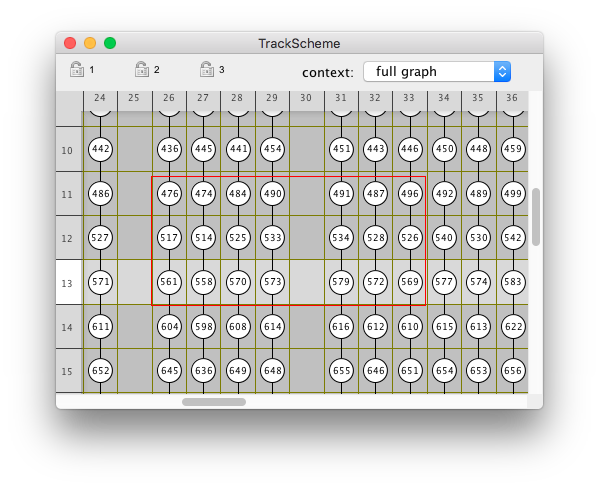
\includegraphics[width=0.35\textwidth,trim=0.5cm .5cm .5cm .5cm,clip]{figures/Mastodon_SelectionBox1.png}}
    \hfill
    \subfloat{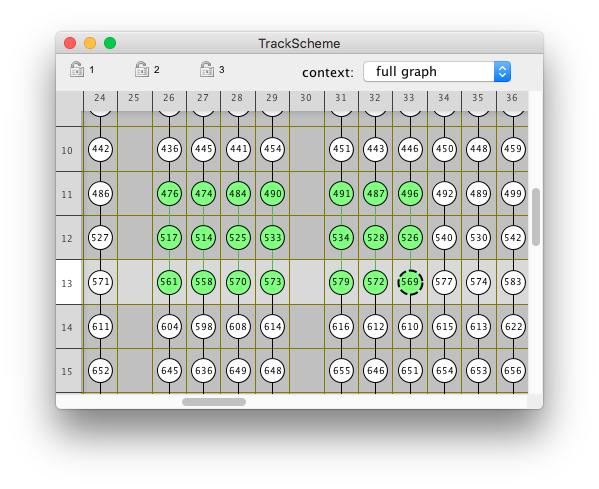
\includegraphics[width=0.35\textwidth,trim=0.5cm .5cm .5cm .5cm,clip]{figures/Mastodon_SelectionBox2.png}}
    \hfill\null
    
    \caption{The selection box in \TrackScheme.}
    \label{fig:SelectionBox}
\end{figure}  



\subsection{Editing spots and links with the selection.}

The selection actions are all applied in bulk. 
You can delete all the spots and the links currently in the selection with \keys{\shift+\backdel}.
If your selection includes spots that are not linked, pressing \keys{\shift+K} will link them sequentially. 
If the selection contains more than one spot per frame, only one of them, picked randomly, will be linked. 



\subsection{Manually adding spots and linking them.}

Adding new spots requires specifying where to add them.
Since \TrackScheme does not include spatial information you cannot use it to add spots.
You can only add spots in the BDV views. 

To add a new spot, simply hover the mouse in a BDV view where you want the spot to be created, and press \keys{A}.
A new spot will appear, with a radius given by the last radius value you used.
You can respectively decrease or increase the radius of a spot by pressing \keys{Q} and \keys{E}.
Modifiers affect the amount of radius changes.
\keys{\shift+Q} and \keys{\shift+E} change the radius by a larger amount and \keys{\ctrl+Q} and \keys{\ctrl+E} by a finer amount.

Spots created this way are not linked. 
It might not be the quicker way to follow manually a cell over several frames. 
To do so, you can use a little trick. 
When you want to add a spot, and link it to an existing one, arrange the BDV view so that this source spot is visible in the displayed time-point.
Then place the mouse cursor \textit{inside} the source spot, and press and hold \keys{A}.
Like for creating links, the BDV moves to the next time-point, paint the source spot and link with white, dashed lines, and let you position the new target spot.
While you keep \keys{A} pressed, you can move the target spot around.
When it is in the desired position, release \keys{A}.
The new spot is created and linked to the source spot.
This way, you can quickly follow a cell or an object and manually creates a track for it by just positioning the mouse with a few presses of \keys{A}.

\subsection{Moving spots around.}

To move an existing spot we use a similar interaction with the spots.
In a BDV view, place the mouse cursor inside the spot you want to move, then press and hold \keys{Space}.
While you hold \keys{Space} pressed the spot will move where you move the mouse. 
Release the \keys{Space} key at the desired location.


\subsection{The undo/redo mechanism.}

One of the most useful actions is undoubtedly undo and redo. 
To undo just press \keys{\ctrl+Z} and to redo use \keys{\ctrl+\shift+Z}. 
There is no limit to the number of undos you can do. 
And everything can be undone in Mastodon, even tag definitions.
In our humble opinion, this is one of the core reasons for Mastodon, a tracking and lineaging software that aims at combining automated and manual approaches, to exist.


\subsection{Putting things in practice.}


\begin{figure}
    \centering
    \null\hfill
    \subfloat[]{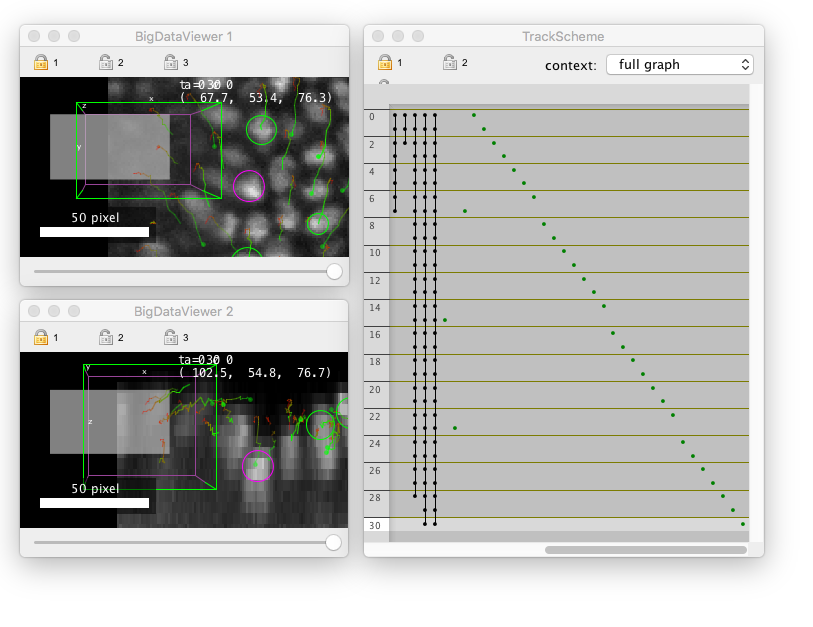
\includegraphics[height=0.18\textheight]{figures/Mastodon_ManualTracking_01.png}}
    \hfill
    \subfloat[]{\includegraphics[height=0.18\textheight,trim=0.5cm .5cm .5cm .5cm,clip]{figures/Mastodon_ManualTracking_02.png}}
    \hfill
    \subfloat[]{\includegraphics[height=0.18\textheight]{figures/Mastodon_ManualTracking_03.png}}
    \hfill\null
    
    \caption{Manual tracking in Mastodon. \textbf{a.}~After selecting the spots we added to each time-point. \textbf{b.}~After linking them with \keys{Shift+K}. \textbf{c.}~Backtracking a cell with \keys{Shift+A}.  }
    \label{fig:ManualTracking}
\end{figure}  



Make sure you have one BDV view and one \TrackScheme view open, and that both are linked using the same lock \smallimg{lock.png}.
In \TrackScheme, select one of the spot or link that belongs to one of the long tracks; the ones that extend from the first time-point to the last.
Press \keys{\shift+Space}.
You selected the whole track to which the spot or link you selected belong to.
Press \keys{\shift+\backdel}.
The track has been removed.

Let's remove a couple of other tracks another way.
Click and drag in \TrackScheme to draw a selection box around some long tracks.
Then press \keys{\shift+\backdel}.
Our model should now lack several good tracks we will try to put back manually.
For clarity, also remove all the tracks on the right part of the \TrackScheme view, that do not start at the first time-point.

In the BDV view, go to the first time-point, and look for a cell whose spot has been removed.
Pan the view (right-click and drag), adjust the zoom (\keys{\ctrl+\shift+Mousewheel}) and the Z position (\keys{Mousewheel} with or without \keys{\shift}) so that the cell is well in view.
Then put the mouse cursor over it and press \keys{A}.
A spot has been added on the cell.
The fine adjustment of the spot position in 3D can be made easier with a second BDV view.
Open another BDV view, zoom and rotate it so that it is aligned with the XZ plane by pressing \keys{\shift+Y}.
Add it to the lock group by toggling the right lock \smallimg{lock.png} in the toolbar.
Go back to the first BDV view, and align it with the XY plane by pressing \keys{\shift+Z}.
You must now find the spot we just added. 
If you cannot find it in any of the two BDV view, look for it in \TrackScheme.
It will be in the rightmost column at the first line, since we added the spot to the first time-point.
Double-clicking on it in \TrackScheme will center the two BDV views on it.
Now that the two BDV views are centered on the spot, you can adjust its XY and Z positions over the cell using the two views.
In any of the two BDV views, put the mouse cursor, then press and hold \keys{Space}.
Move the spot the desired location and release \keys{Space}.
The spot might not have the right diameter to encompass the cell.
Change its radius by pressing \keys{\shift+Q} and \keys{\shift+E} (without \keys{\shift} for finer adjustments) until you are happy with it.

You must now do it for the same cell in the subsequent time-points.
Press \keys{M} in a BDV view to move to the next time-point.
Again, put the mouse cursor roughly at the center of the cell and press \keys{A}.
Adjust its position with \keys{Space} and move to the next time-point.

We have to repeat this for all the time-points of the movie (Figure~\ref{fig:ManualTracking}a).
This might be tedious but does not have to be too long. 
When I need to do this I adopt a posture similar to what I have when I play PC video-games: the right hand on the mouse, the left hand over the left side of the keyboard, over the \keys{A}, \keys{D}, \keys{Q}, and \keys{E}.
The \keys{\shift} key can be accessed with the little finger, the \keys{Space} key with the thumb.
The \keys{N} and \keys{M} keys to navigate over time are accessible with the left thumb also.

We created a bunch of spots, but they are not linked. 
Move to the \TrackScheme view. 
You will find the spots you last created there always at rightmost part of the view.
Since they are not linked, they should appear each in their separate column, in a stairway manner. 
Select them all by dragging a selection box around them and press \keys{\shift+K}.
They should now link together into a new track (Figure~\ref{fig:ManualTracking}b).
With one of the spot of this newly created track selected, press \keys{\Alt+\arrowkeyup} to jump to the first spot in the track.
Then press \keys{\return} to edit its name into something like \texttt{My first track}.

We can create a track directly.
Let's do this by backtracking a cell from the last time-point to the first.
In a BDV view, move to the last time-point, and place the mouse cursor over an annotated cell. 
Create a spot over it by pressing \keys{A} and center and resize it until satisfaction.
Now keep the mouse cursor inside this spot, and press \keys{\shift+A} and hold the \keys{A} key.
The BDV view moves to the previous time-point and creates a new spot there, already linked to the other one.
By repeating this you can create a track that will backtrack the cell until it appears in the movie (Figure~\ref{fig:ManualTracking}c).

We have now restored two of the tracks we removed at the beginning of this paragraph.
Hopefully now you feel enough at ease to do these manipulations quickly, efficiently and without too much hassle.
But one of the concluding beauty of this chapter is that you can restore the data as we had it at the beginning by roughly 100 presses of the \keys{\ctrl+Z} keys.


\newpage
\section{Getting your bearings in large datasets.}

In the previous chapter we have seen how to edit single spots and links within a Mastodon model.
As we said before, the goal of Mastodon is to let you harness very large images, for which the number of annotations can be very large too.
It can be very easy to get lost within such large images and loose track of where we are within the sample image and what cell we follow. 
So we have added several features that are made especially to get your bearings in large datesets.
More than anything, these features are about giving visual cues that ease orientation, and exploit event that a human eye would consider salient. 
We took some inspiration from video-games, that are very good at communicating condensed and synthetic information to the player
(but only for a limited part; there is no screenshake when you delete a spot).



\subsection{Bookmarks in the BDV views.}

\subsection{Linking several views together.}

\subsection{In Mastodon everything is animated.}

\subsection{Spatial context in TrackScheme.}

\newpage
\section{Numerical features and tags. The table view.}

Mastodon is a tracking and lineaging tool.
Its output is a collection of tracks, and the analysis of these tracks to yield statistics on \eg velocity, displacement \etc is carried out in another software package such as MATLAB or Python.
Nonetheless you will find in Mastodon tools to compute \textit{numerical features} on data item. 
Numerical features are numbers that can be calculated on spots, links and tracks of the data. 
For instance there are feature for the number of links that touch a spot, or the displacement of a link or the number of spots in a track.
You can find them within Mastodon because it is convenient, but also because they are very useful for the interactive exploration of your data. 
Coupled with feature-based coloring, the display and sorting of values in the table view and the selection creator tool, they can considerably accelerate and facilitate making sense of the data.

Numerical features are numbers that classically relate to a physical quantity.
When we need to \textit{categorize} items, we rely on \textit{tags}.
We describe them just below. 
This chapter will also show you how to compute numerical features and create a coloring view from the feature values and  tags.
Doing so, we will introduce the third kind of data view in Mastodon: the data tables.


\subsection{Tags and tag-sets.}

As we said above, every-time you need to categorize certain data items, or need to visualize categories, you should rely on tags.
Let's suppose that you are investigating the trajectories of cells in a developing embryo from an early stage to a stage where the embryo is polarized.
Some cells will migrate to the anterior part, some others to the posterior part, \etc. 
You might want to tag cell tracks with the \texttt{Anterior} or \texttt{Posterior} tag, to investigate where do these cell come from in the early embryo.
Or let's say that you are curating the results of the automated tracking on a large images. 
The tracking results might have some inaccuracies, and you want to correct them for important tracks.
Because there is a lot of tracks, you share the workload with some colleagues. 
You work asynchronously with them, editing the Mastodon file one after another. 
Doing so, you can use tags in Mastodon to mark some tracks as reviewed by you.
Your colleagues will use a tag for themselves, to ensure that no two scientists are reviewing the same track twice.
All the cells that are not tagged in this categorisation are still waiting to be reviewed. 

In Mastodon, a categorization corresponds to a \textbf{tag-set}.
A tag-set defines a property that can have a reasonable number of discrete values, or \textbf{tags}.
In the first of the two examples above, \texttt{Location} would be a tag-set to specify the location of cells.
\texttt{Anterior} and \texttt{Posterior} would be two tags belonging to the \texttt{Location} tag-set.
In the second example, \texttt{Reviewed by} would be a tag-set, and \texttt{Mette}, \texttt{Pavel}, \texttt{Tobias} and \texttt{Jean-Yves} would be 4 tags of this tag-set.

You can assign tags to spots and links.
To assign a tag to a whole track, you have to assign this tag to all the spots and links of this track.
One data item (a spot or a ling) can have 1 or 0 tags per existing tag-set.
But they can be categorized by as many tag-sets as there is.
For instance, a spot can have the tag \texttt{Anterior} in the \texttt{Location} tag-set, and the tag \texttt{Pavel} in the \texttt{Reviewed by} tag-set. 
Or it can be not tagged in the \texttt{Reviewed by} tag-set.
But it cannot have both the tag \texttt{Mette} and the tag \texttt{Tobias} because they belong to the same tag-set.
Each tag-set works independently, and clearing a tag-set does not affect the others even for one data item.
Now that we set things straight, let's see how to create tag-sets.
We will base the demonstration in this chapter on the data we generated in the tutorial chapter~\ref{Getting_started}.


\subsubsection{Creating tag-sets.}

On the main window (see figure~\ref{fig:MastodonMainWindow} page~\pageref{fig:MastodonMainWindow}), there is a button \menu{configure tags}. 
Pressing it opens the tag-set dialog. 
Right now, it appears as an empty table made of two columns (Figure~\ref{fig:CreateTagSet}a). 
This is where you enter tag-sets and tags.

Press the \smallimg{add.png} button on the left column to create a new tag-set. 
A default name is shown for the tag-set, that you can edit.
You can also directly press the  \keys{\return} key to immediately start editing the new tag-set.
Let's say we want to create the location tag we talked about before.
Type \texttt{Location} in the text field. 
An empty line followed by a \smallimg{add.png} button should appear on the right column.
This is where you will enter the tags of this tag-set.
Click on this button, or press the \keys{\tab} key followed by the \keys{\return} key to create a new tag.
For instance, the \texttt{Anterior} tag.
Note that a tag is only made of a label (the text) and a color.
The color will be used in Mastodon views.
Create a second tag for the same tag-set called \texttt{Posterior}.
Pick the color as you like. 
Now try to create another tag-set called \texttt{Reviewed by} and create some tags in this tag-set (Figure~\ref{fig:CreateTagSet}b). 
The tag-set dialog is normally fully navigable with the \keys{\tab}, \keys{\arrowkeyup} and \keys{\arrowkeydown} keys, so that you can enter tags quickly if you have a lot of them.
You can create new tag-set or new tags with the \keys{\return} key, and delete them either with the \keys{\del} key or by pressing the \smallimg{delete.png} button.

When you are finished, press the \menu{OK} button.


\begin{figure}
    \centering
    \null\hfill
    \subfloat[]{\includegraphics[height=0.15\textheight]{figures/Mastodon_ConfigureTagSet_1.png}}
    \hfill
    \subfloat[]{\includegraphics[height=0.15\textheight,trim=0.5cm .5cm .5cm .5cm,clip]{figures/Mastodon_ConfigureTagSet_2.png}}
    \hfill\null
    
    \caption{Creating tag-sets and tags. \textbf{a.}~The empty tag-set dialog. \textbf{b.}~After adding two tag-sets and six tags.  }
    \label{fig:CreateTagSet}
\end{figure}


\subsubsection{Assigning tags to data items.}

Tags are set via the selection tool, presented above (chapter~\ref{Selection_tool} page~\pageref{Selection_tool}).
Once you have some spots and links in the selection, you can assign a tag to it via the \menu{Edit > Tags > The tag set name > The tag label} menu.
The menu content will be updated with the tag-sets and tags you defined in the tag-set dialog, described above (Figure~\ref{fig:AssignTagSetMenu}).
This will work in any Mastodon views, BDV or \TrackScheme.

\begin{figure}
    \centering
    \includegraphics[height=0.2\textheight]{figures/Mastodon_ColorByTagSet_1.png}
    
    \caption{The menu item to assign tag-sets and tags to the current selection. }
    \label{fig:AssignTagSetMenu}
\end{figure}


\TrackScheme ships a second way to set tags quickly from the keyboard.
After selecting the spots and links of interest, press the \keys{Y} key.
A floating menu should appear on the left part of the view panel (Figure~\ref{fig:AssignTagSetShortcut}). 
There is a bit of naming clash in the floating menu.
Here, tag-sets are called \textit{tags} and tags are called \textit{labels}.
Select the desired tag-set with the \keys{1}, \keys{2}, .. keys.
The menu now shows the tags defined within this tag-set, that you can select the same way.
Note that there is a way to remove all the tags over all the tag-sets on the selection by pressing \keys{\shift+\del} on the first menu, or just the tags of the selected tag-set by pressing \keys{0} on the second menu.


\begin{figure}
    \centering
    \null\hfill
    \includegraphics[height=0.2\textheight]{figures/Mastodon_ColorByTagSet_2.png}
    \hfill
    \includegraphics[height=0.2\textheight,trim=0.5cm .5cm .5cm .5cm,clip]{figures/Mastodon_ColorByTagSet_3.png}
    \hfill\null
    
    \caption{Assigning tags in \TrackScheme. After pressing the \menu{Y} key this floating menu is shown, that can be navigated with the digit keys.  }
    \label{fig:AssignTagSetShortcut}
\end{figure}



\subsubsection{Coloring views by tag-sets.}

The tags we just defined and assigned can be used in with the views, to highlight the items that are tagged. 
In the \menu{View > Coloring} menu of any view in Mastodon, you will find a sub-menu updated with the tag-sets you created among other choices (Figure~\ref{fig:ColorByTagSetMenu}). 
By default, newly created views are colored with the \menu{None} coloring mode, which simply colors all the spots and links the same way, taking colors from render settings. 
If you select a mode corresponding to a tag-set, tagged spots and links will appear painted with the color you chose for the tags of this tag-set (Figure~\ref{fig:ColorByTagSetTrackScheme}).
This is very handy to mark some locations in the image or highlight interesting tracks in the data.
Later we will see that tags can be used to retrieve specific items for further processing.
Finally, in \TrackScheme there is an option to show a legend of the current coloring mode.
You can toggle it on or off and set the location of this legend in the \menu{View > Colorbar} menu.

\begin{figure}
    \centering
    \includegraphics[height=0.1\textheight]{figures/Mastodon_ColorByTagSet_4.png}
    
    \caption{The coloring menu, updated with the tag-sets. }
    \label{fig:ColorByTagSetMenu}
\end{figure}

\begin{figure}
    \centering
    \includegraphics[height=0.25\textheight]{figures/Mastodon_ColorByTagSet_5.png}
    
    \caption{Coloring with tag-sets in \TrackScheme. }
    \label{fig:ColorByTagSetTrackScheme}
\end{figure}


\subsection{Numerical features.}

Numerical features are values that are calculated from the data.
For instance the mean intensity within a spot, or the displacement along a link.
They are very generic: the main restrictions is that there must be a data item (a spot or a link) per feature value. 
But the feature itself can be scalar, non-scalar, real, integer, a string, a vector, 
\etc.
They are \textit{labile}. 
Because they are defined for a data item, they will become invalid as soon as the data item changes.
Think of what happens to the spot mean intensity if the spot is moved over the image for instance.
Because we want to accommodate extensibility and large data, we have to use a special system that we describe below. 

\subsubsection{Feature computation.}

Numerical feature values are calculated by \textbf{feature computers}.
Feature computers are actually specialized Mastodon plugins, made so that it is easy for a 3rd party (you) to implement their own features in Mastodon.
We explain you to write your own feature computer in the second part of this manual, dedicated to technical information.

Because feature computation can take very long on large images, you have to trigger it manually.
On Mastodon main window, you can find a button \texttt{compute features} button.
Pressing it will show the feature computation dialog (Figure~\ref{fig:FeatureComputationDialog}).
The feature computers are listed on the left panel.
Clicking on the computer name displays some information about the feature they compute in the right panel. 
Note that they are named 'features' on this panel, but they are in reality the feature computers.
For instance if you click on the \texttt{Spot gaussian-filtered intensity}, you will see in the information panel that this computer generates a feature for the mean intensity (weighted by a gaussian) and its standard deviation within a spot.
Note also that they can have dependencies.
For instance, the \texttt{Link velocity} feature computer depends on the \texttt{Link displacement} feature to be present at the time of computation.

\begin{figure}
    \centering
    \includegraphics[height=0.3\textheight]{figures/Mastodon_FeatureComputation_1.png}
    
    \caption{The feature computation dialog. }
    \label{fig:FeatureComputationDialog}
\end{figure}

The check-box on the left of each feature computer name triggers whether they will be part of the next feature computation.
Press the \menu{\smallimg{bullet_green.png}Compute} button to trigger computation of features.
You will probably notice, thanks to the progress bar, that the intensity-related features are the ones that take the most time to compute. 

Once the computation of all the features is complete, all the small clock icons that were shown right to the feature computer names now turned to a green dot\smallimg{bullet_green.png}.
This is how we keep track of the validity of the feature values.
Since the feature computation is triggered manually, and that a feature value might invalidated if the data changes (new spots added, removed, moved, changed the radius, added or removed some links), this icon serves as a signal for feature value de-synchronization.     
If the icon is shows as a clock~\smallimg{time.png}, it means that the data changed since the last feature computation, and that the feature values are out of sync. 
If is shows a green dot\smallimg{bullet_green.png}, then the data did not change since last computation, and the feature values are sure to be valid. 
This is very important for proper interpretation of the data, and you will have to show the computation dialog often just to check the feature values validity. 
By the way, you can check now how the validity flag works. 
While keeping the feature computation dialog open, move a spot in a BDV view. 
You should see that all the green dot icons now turn to the clock icon.
Also, if you now deselect some feature computers before launching a new computation, the validity flag will not turn to the green dot icon for those feature computers.

I guess that since we have feature values computed, you would like to inspect them and export them for further analysis.
This is the role of the table view, but before getting to it, we will make a little detour to showing how to use features to generate coloring, accelerating updates of computation and saving them to disk.


\subsubsection{Coloring views by numerical features.}
\label{Configure_Color_Modes}

We have seen above that tag-sets could be used to generate coloring of the data items shown in a view. 
Indeed, in the \menu{View > Coloring} menu of each view, that tag-sets are listed and when selected, are used to assign a color to each data item.
We can do something similar with feature values, except that feature based coloring requires more input from us.

Feature color modes need to be created first, and this is done in a dedicated user interface. 
Select the \menu{File > Preferences} menu item in the main window or any view.
The preferences dialog is shown.
It is organized with a side-bar on the left that contains the various items that can be configured in Mastodon. 
Parenthetically, you can see that you can configure the display style of the \TrackScheme and BDV views, and the keymaps. 
But we will see this later.
In the sidebar select \menu{Feature Color Modes}.
The panel on the right now display the feature color mode configuration panel (Figure~\ref{fig:FeatureColorModeConfig1}).

Its top line has a drop-down list that contains all the color modes already defined. 
Right now, there is only one, called \textbf{Number of links}.
As the \textbf{\textit{built-in}} suffix indicates, it is a built-in color modes, and it cannot be edited. 
To create a new one you must duplicate it and rename the new one.   
Do so by clicking on the \menu{Duplicate} button, then on \menu{Rename}.
Let's create a color mode that color spots and links based on the mean intensity inside the spots, that we would call \textbf{Mean intensity}.

\begin{figure}
    \centering
    \includegraphics[height=0.3\textheight]{figures/Mastodon_FeatureColorModeConfig_1.png}
    
    \caption{The feature color mode configuration preference dialog. }
    \label{fig:FeatureColorModeConfig1}
\end{figure}

The rest of the configuration panel is made of two parts.
The top part configures the vertex coloring, or how we color spots.
The bottom part configures the edge coloring, or how we color links. 
In Mastodon the data is organized in a mathematical graph\footnote{\href{https://en.wikipedia.org/wiki/Graph_(discrete_mathematics)}{Mathematical graphs on Wikipedia \coloredlink{https://en.wikipedia.org/wiki/Graph\_(discrete\_mathematics)}}}, in which the vertices are the spots, and the edges are the links that connect spots from one frame to another, so you will sometimes find in Mastodon and in this manual the vocables vertex and edge to design a spot and a link respectively. 
The vertex color mode specifies where do we take colors from. 
You can choose between:
\begin{myitemize}
    \item \texttt{Vertex}, which means a spot will take its color from a feature value it owns.
    \item \texttt{Incoming edge}, which means a spot will take its color from a feature value owned by the single incoming link that targets this spot. This is the link backward in time. If there are no such links or more than one, then the default color is used.
    \item \texttt{Outgoing edge} is the same thing, but for the link forward in time. 
    \item \texttt{Default} mode does not rely on feature values but simply uses the default color in the view.
\end{myitemize}

\noindent Depending on the mode you chose, the content of the drop-down list below, called \texttt{Vertex feature}, will change to reflect either the list of spot features or the link features.
Select \textbf{Vertex} as a color mode and \textbf{Spot gaussian-filtered intensity} as feature.
Two new drop-down list appear on the right of the feature list. 
One contains the list of projections in the feature and the second one contains the list of channels in the dataset. 

We need to explain a bit what are \textbf{feature projections}.
We said above that a feature could be roughly anything numerical, and was not necessarily a scalar. 
It could be a vector, a tensor, a complex number, \etc.
However to be usable and useful in Mastodon, features are required to expose a sensible list of projections that compose them.
Feature projections are scalar and real values that can decompose or project a feature on a real axis.
How they are defined is up to the person that created the feature computer, but we can rely on the \textit{hope} that they choose wisely. 
For instance, a feature that gives the velocity vector of a link will reasonably expose 3 projections, one for each of the X, Y and Z component of the vector. 
Or maybe the polar angle, azimuthal angle and norm of this vector.
Or maybe the 6 projections since they can be calculated on the fly. 
A complex feature value will reasonably expose 2 projections, one for the real part, one of the imaginary part.
\textit{Etc}.
The \texttt{Spot gaussian-filtered intensity} feature has two projections, one for the mean value of the intensity within a spot and the standard deviation of this intensity.
Since both can be computed on any of the channel present in the dataset, their number is multiplied by the number of channels. 
The configuration panel changes according to the number of projections in a feature and its multiplicity (Figure~\ref{fig:FeatureColorModeConfig2}). 
For features that are made of one real value with no multiplicity, the projection list is superfluous and not shown.
In our case, we simply want the mean of the only channel in the dataset.

Coming back to the color mode configuration, next we need to pick a color-map.
A color-map acts as the LUT for an image, and maps a color to a certain value. 
Mastodon ships about 20 of them, many taken from the MatPlotLib project\footnote{\url{https://matplotlib.org/3.1.1/gallery/color/colormap_reference.html}}.
Finally, you have to specify a min value and a max value that will act as the brightness and contrast values for an image.
Values below the min you defined will all be displayed with the first color of the color-map and values larger than the max with last.
The black square you see next to the graded representation of the color-map is the color used for data items for which the feature value is not present or undefined (division by zero, \etc).
The \texttt{autoscale} button computes the min and max automatically from the feature currently selected with the values taken from the last feature computation.

The edge coloring works exactly the same, except for the edge color mode.
\begin{myitemize}
    \item \texttt{Edge} means that a link will be colored by a feature value it owns.
    \item \texttt{Source vertex} will take a feature value from the source spot of this link, that is, the first in time.
    \item \texttt{Target vertex} does the same but for the last spot in time of this link. 
    \item \texttt{Default} mode does not rely on feature values but simply uses the default color in the view.
\end{myitemize}
\noindent To build our example feature color mode, choose \texttt{Source vertex} as color mode, and use for instance the \texttt{viridis} color-map along with 700 and 1100 for min and max values.
Do the same for the vertex color mode (Figure~\ref{fig:FeatureColorModeConfig2}).


\begin{figure}
    \centering
    \includegraphics[height=0.3\textheight]{figures/Mastodon_FeatureColorModeConfig_2.png}
    
    \caption{Our custom feature color mode, based on spot intensity. }
    \label{fig:FeatureColorModeConfig2}
\end{figure}

Like for tag-sets, the \menu{View > Coloring} menu is now updated with items corresponding to the color modes we created.
If they are grayed-out, it means that the feature values they depend on is not yet computed.
This kind of view immediately reveals important aspect of the data, even at a very high level.
For instance with our custom color mode, we can quickly find cells that are the brightest, and visually inspect how the intensity in cells change over time (Figure~\ref{fig:FeatureColorModeView}).

\begin{figure}
    \centering
    \null\hfill
    \includegraphics[height=0.23\textheight]{figures/Mastodon_FeatureColorBDV.png}
    \hfill
    \includegraphics[height=0.23\textheight]{figures/Mastodon_FeatureColorTrackScheme.png}
    \hfill\null
    
    \caption{Feature color mode in a BDV view and in a \TrackScheme view.  }
    \label{fig:FeatureColorModeView}
\end{figure}




\subsubsection{Accelerating feature computation with the update mechanism.}

In this paragraph we explain one of the important aspect of feature computation in Mastodon, in the case of large data.
It is not an interactive tutorial, but what it covers deserves explanation. 

As we repeated several times in this manual, Mastodon is meant to harness large images and large data generated from it. 
You probably noticed that the feature computers that deal with spot intensity (\texttt{Spot gaussian-filtered intensity}, \texttt{Spot median intensity}, \texttt{Spot sum intensity}) were taking a long time to compute. 
They require synchronized access to pixel data, jumping from one spot to another, at a fixed resolution level.
In situations where you have millions of spots, the computation of these features will take a very long time, possibly similar to the time it took to detect these spots. 
So of course, you don't want to do it again and again each time one spot changes radius or position.
You want to recompute feature values only for the spots that have been altered or created since the last computation. 
Mastodon has a system that supports incremental updates. 
This system tracks what data items have been modified or created for a given number of feature computation times. 
It feature an \textit{update stack} that can provide to the feature computer that request it the list of data items that changed since the feature it provides have been last computed (Figure~\ref{fig:FeatureUpdateStack}). 

You can it a try with a larger dataset than the one we have been using so far.
Compute all the features, including the costly ones such as \texttt{Spot gaussian-filtered intensity}.
The first time you compute this features, it should take a significant amount of time.
Now move one spot from one position to another, and recompute all the features. 
You should see that now the computation takes much less time.

\begin{figure}
    \centering
    \includegraphics[angle=90, height=0.8\textheight]{figures/Mastodon_FeatureUpdateStack.png}
    \caption{An illustration of the feature update stack mechanism.  }
    \label{fig:FeatureUpdateStack}
\end{figure}


\subsection{Tags, numerical features and saving the data to disk.}

All tags and feature values are saved in the Mastodon file. 
The feature update stack state is saved too, so you will retrieve everything back as it was when you saved.
We did not have a choice, it was the only reasonable way to achieve a usable feature and tag framework in the case of very large data.


\subsection{The data table views.}
\label{sec:DataTables}

\subsubsection{The main table view.}

The BDV and \TrackScheme views are not suitable to display all the feature values we computed.
The coloring we have been using with them is good only for visualization purpose. 
There is a nice view to properly inspect and exploit feature values in subsequent steps in your analysis: the table view.
In practice, the table view is simply a tabular representation of the data items in Mastodon.
Spots and links are displayed in a list where a single row corresponds to a data item, and columns to feature values and tags. 
You can create a new table view by using the menu \menu{Window > New data table}.
If you did not compute features and did not define and tag-set, it should look like the table in figure~\ref{fig:TableViewEmpty}.
The view is made of two tables, one for spots (\texttt{Vertices} pane) and one for links (\texttt{Edges} pane).
Right now it is pretty empty. 
The spot and link tables only show the label and ID of the spots.
Navigating in this table is done classically: the arrow keys \menu{\arrowkeyup} and \keys{\arrowkeydown} jump from one row to the next, and \keys{\arrowkeyleft} and \keys{\arrowkeyright} from one column to the next.
\keys{Page\ \arrowkeyup} and \keys{Page\ \arrowkeydown} jump page per page.
\keys{\ctrl + Page\ \arrowkeyup} and \keys{\ctrl + Page\ \arrowkeydown} alternate between the spot table and the link table.

\begin{figure}
    \centering
    \null\hfill
    \includegraphics[height=0.23\textheight]{figures/Mastodon_TableView1.png}
    \hfill
    \includegraphics[height=0.23\textheight]{figures/Mastodon_TableView2.png}
    \hfill\null
    
    \caption{The table view, with no features computed and no tags defined. Left: the table for spots (\texttt{Vertices} pane). Right: the table for links (\texttt{Edges} pane).  }
    \label{fig:TableViewEmpty}
\end{figure}

After computing some features and defining some tag-sets, the table show new columns (Fi\-gu\-re~\ref{fig:TableViewFeatureTags}). 
Note that the column headers represent the feature with their projection and physical units on several rows.
For instance, the \texttt{Spot gaussian-filtered intensity} feature name is displayed on the first row of the column header.
The header is split in two columns on the second row, one for each projection included in the feature (mean and standard deviation of a single channel).
And in the third and last row, the units of each projection is display in brackets (Counts in this case).
The header of the tag-set columns are similar.
The first row shows the name of the tag-set, and the second row shows each of the tag the set contains, with the tag chosen color as background.

\begin{figure}
    \centering
    \includegraphics[height=0.27\textheight]{figures/Mastodon_TableView3.png}
    
    \caption{The table view, with features and tags.  }
    \label{fig:TableViewFeatureTags}
\end{figure}

The table view can be used to edit in part the data  (Fi\-gu\-re~\ref{fig:TableViewEditing}). 
For instance you can edit the spot label directly in the table. 
Just navigate to the row of spot you want to change the name of and the \texttt{Label} column, then press \keys{F2}.
The label field becomes editable.
When you are done editing, press \keys{\return}.
The tags are displayed as check-boxes in the table, that you can set directly by clicking on them.
Or you can navigate the desired row and column and set them with the \keys{Space} key.

\begin{figure}
    \centering
    \includegraphics[height=0.27\textheight]{figures/Mastodon_TableView4.png}
    
    \caption{After editing spot labels and tags.  }
    \label{fig:TableViewEditing}
\end{figure}

The highlight and selection are also shared with table views. 
When the table view is not active, selected items are shown with a gray background.
The highlight spot or link is shown in the table with a thick black border (Figure~\ref{fig:TableViewHighlightSelection}).
To add rows to the selection, the default key-bindings are again standard.
Press \keys{\shift+Left-click} to add a range of rows to the selection from a rable view, or use \keys{\shift+\arrowkeyup} or \keys{\shift+\arrowkeydown} or \keys{\shift+Page\ \arrowkeyup} and \keys{\shift+Page\ \arrowkeydown}.
By pressing \keys{\ctrl+Left-click} or \keys{\cmd+Left-click} you can toggle single rows in and out of the selection.
Of course, all of the commands related to the selection we have seen before also apply to the table views (Table~\ref{tab:MastodonSelectionKeys} page~\pageref{tab:MastodonSelectionKeys}).


Another feature of data tables is that they can be made slave of a spatial context, like for \TrackScheme.
When another BDV view is active, you can select its name in the drop-down list on the top-right part of the table. 
Then the table only shows the data items that are currently displayed in the master BDV view.
The notion of spatial context is explained above (section~\ref{sec:SpatialContext} page~\pageref{sec:SpatialContext}).
See also the figure~\ref{fig:SpatialContext} page~\pageref{fig:SpatialContext}.

\begin{figure}
    \centering
    \null\hfill
    \includegraphics[height=0.23\textheight]{figures/Mastodon_TableView5.png}
    \hfill
    \includegraphics[height=0.23\textheight]{figures/Mastodon_TableView6.png}
    \hfill\null
    
    \caption{Highlight and selection in the table view.  }
    \label{fig:TableViewHighlightSelection}
\end{figure}

\subsubsection{Sorting rows.}

The table can be sorted by clicking on the header of the column you want to use for sorting. 
It works for labels, IDs, feature values and tags

\subsubsection{The selection table.}

There exists a variation of the table view, but that display only what is currently in the selection.
To display such a table, go to \menu{Window > New selection table} in the menu.
The selection table that appears only shows what is in the selection, and is constantly updated to reflect changes in the selection (Figure~\ref{fig:SelectionTable}).
You cannot use it to edit the selection like in the main table.
However the row you pick in this table will set the focus and highlight in other views.
Everything else applies to the selection table.

\begin{figure}
    \centering
    \null\hfill
    \includegraphics[height=0.23\textheight]{figures/Mastodon_TableView7.png}
    \hfill
    \includegraphics[height=0.23\textheight]{figures/Mastodon_TableView8.png}
    \hfill\null
    
    \caption{The selection table.  }
    \label{fig:SelectionTable}
\end{figure}

\subsubsection{Feature-based coloring in table views.}

Of course, feature based coloring works with the table views (Figure~\ref{fig:TableViewFeatureColoring}).
And it can give a pleasant display when combined with sorting rows by a feature column.


\begin{figure}
    \centering
    \includegraphics[height=0.27\textheight]{figures/Mastodon_TableView9.png}
    
    \caption{Feature-based coloring in table views.  }
    \label{fig:TableViewFeatureColoring}
\end{figure}

\subsubsection{Exporting table data.}

The data currently displayed in a table view can be exported to CSV.
When a table window is active, select the menu item \menu{File > Export to CSV}.
You will have to specify a saving location and a name.
But two CSV files will be produced: one for the spot table (appended with \texttt{-vertices.csv}) and one for the link table (appended with \texttt{-edges.csv})
Only the data currently displayed in the view are saved, and ordered as in the view. 
This means that if you call the \menu{File > Export to CSV} command from a selection table, only the current selection will be saved.


\begin{table}[!htbp]
    \centering
    
    \caption{Default navigation key-bindings for Mastodon-table views.}

    \begin{tabulary}{\textwidth}{L|J}
    
    \toprule
    \textbf{Action}                 & \textbf{Key}              
    \\ \midrule
    
    \multicolumn{2}{c}{\textit{Navigation.}}
    \\ \midrule
    
    Move from row to row             & \keys{\arrowkeyup} and \keys{\arrowkeyup}.
    \\ \midrule
    
    Move column to column            & \keys{\arrowkeyleft} and \keys{\arrowkeyright}.
    \\ \midrule

    Display the spot table / the link table            & \keys{\ctrl + Page\ \arrowkeydown} and \keys{\ctrl + Page\ \arrowkeyup}.
    \\ \midrule

    \multicolumn{2}{c}{\textit{Editing.}}
    \\ \midrule
    
    Edit spot label                & \keys{F2} when focus is in the label column.
    \\ \midrule

    Toggle tag                      & \keys{Space} when focus is in the desired tag column.
    \\ \midrule
    
    \multicolumn{2}{c}{\textit{Selecting.}}
    \\ \midrule
    
    Add next / previous row to selection        & \keys{\shift+\arrowkeyup} and \keys{\shift+\arrowkeydown}
    \\ \midrule

    Add range to selection        & \keys{\shift+Page\ \arrowkeyup} and \keys{\shift+Page\ \arrowkeydown} or \keys{\shift+Left-click} 
    \\ \midrule

    Toggle row into selection        & \keys{\ctrl+Left-click} or \keys{\cmd+Left-click} 
    \\ \bottomrule

\end{tabulary}


    \label{tab:MastodonTableKeys}
    \vspace{-10pt}

\end{table}


\newpage
\section{Semi-automated tracking.}

Let us suppose we are dealing with a difficult image in which me must track only a subset of cells. 
The cells are difficult to track automatically, for instance because there are many spurious structures labelled. 
Or because there are other cells of different sizes in the tissue we are studying. 
Or because the image quality varies in time and space. 
The data is such that that fully automated algorithms introduced in chapter~\ref{Getting_started} won't give us fully accurate results. 
We can use the manual editing tools introduced in chapter~\ref{Manuel_Editing} and curate the results of automated tracking, removing spurious detections and links, and fixing incorrect ones. 
Another approach would be to start from a blank annotation and track manually only the cells we are interested in. 
Both approaches might be long and tedious. 
We introduce in this chapter tools for semi-automated tracking, that should alleviate the work of the second approach.

Semi-automated tracking is simply a way of following a specific cell that you picked-up manually. 
The tracker will follow the cell over time, and create spots and links for a certain amount of time-points.
It searches for the best location candidate in the next time-point around the location of the spot.
It then creates a new spot there and links it to the previous one.
This procedure is repeated this for a certain number of time-points you can set, creating or augmenting a track starting from the spot you selected.

The semi-auto tracker can be configured to work backward in time (backtracking), to have a certain search radius, or a certain sensitivity to spot quality (as defined in chapter~\ref{Detecting_Cells}).
The way it interacts with existing annotation can be configured too. 
You can make it stops when it meets an existing spot, linking to it or not.
You can make it connect to small tracks and resume tracking when it meets the track end.
You can force it to only create links on already existing spots. 
These configuration options give rise to several use-cases we will also survey in this chapter.
But the important message is that semi-automated tracking is a convenient means for dealing with difficult cases, when a fully automated approach fails, and when the data to track is large that doing it manually is inconvenient.

\subsection{Simple semi-automated tracking.}

We will introduce semi-automated tracking on a movie with empty annotation. 
Open the dataset we have been using so far, and clear all annotations (for instance select all \keys{\ctrl+A} then delete selection \keys{\shift+\backdel}).
Then pick a cell in the top layer, and create a spot, centered on its brightest part, like for instance on Figure~\ref{fig:BeforeSemiAutoTracking}.
Adjust its radius and select it.

\begin{figure}
    \centering
    \null\hfill
    \includegraphics[width=0.3\textwidth]{figures/Mastodon_SemiAutoTracking_01a.png}
    \hfill
    \includegraphics[width=0.3\textwidth]{figures/Mastodon_SemiAutoTracking_01b.png}
    \hfill\null
    \caption{Manually picking a cell for semi-automated tracking.}
    \label{fig:BeforeSemiAutoTracking}
\end{figure}

To start semi-automated tracking, press \keys{\ctrl+T}.
A log window should open, and tracking should proceed. 
If the log does not complain about candidates being too far, you should end up with something resembling Figure~\ref{fig:AfterSemiAutoTracking}.
The tracking stopped after 10 frames, and the last spot added is now in the selection. 
Each spot is centered on the cell we started with, and it has the same radius that of the first spot we created. 
You can resume semi-automated tracking from the last spot created by just pressing \keys{\ctrl+T} again. 
If you do it one more time you should reach the end of the movie, with a new track following a single cell over the full movie duration.
To get it, you just had to press \keys{\ctrl+T} 3 times.

\begin{figure}
    \centering
    \null\hfill
    \includegraphics[width=0.2\textwidth]{figures/Mastodon_SemiAutoTracking_02.png}
    \hfill
    \includegraphics[width=0.4\textwidth]{figures/Mastodon_SemiAutoTracking_03.png}
    \hfill\null
    \caption{Results of semi-automated tracking.}
    \label{fig:AfterSemiAutoTracking}
\end{figure}



\subsection{Configuring the semi-automated tracker.}

\subsection{Main use-cases for semi-automated tracking.}

\subsubsection{Tracking from a blank annotation. }

\subsubsection{Patching small track segments.}

\subsubsection{Backtracking, branching on cell divisions. }

\subsubsection{Sparse linking over dense spots.}



\newpage
\part{Technical information.}

\newpage
\bibliographystyle{plainnat}
\bibliography{References}









\end{document}
% vim::set expandtab tabstop=4 softtabstop=2 shiftwidth=2 ft=tex:
